% HTML source for the September 2026 posted paper.
% Body exported from the saved LyX source; print layout is supplied by the site.
\documentclass[11pt]{article}
\usepackage[T1]{fontenc}
\usepackage[utf8]{inputenc}
\usepackage{amsmath,amssymb,amsthm,mathrsfs}
\usepackage{graphicx,booktabs,array,caption}
\usepackage{setspace,placeins}
\usepackage[authoryear]{natbib}
\usepackage{hyperref}
\urlstyle{same}
\newcolumntype{d}[1]{r}
\newtheorem{theorem}{Theorem}
\newtheorem{sectiontheorem}[theorem]{Theorem}
\newtheorem{corollary}{Corollary}
\newtheorem{proposition}{Proposition}
\begin{document}












\section{Introduction}\label{sec:introduction}

As agentic AI models grow more powerful, many workers fear AI is
coming for their jobs. They worry that AI-driven growth will immiserate
them. The fear is not difficult to understand: as agentic AI becomes
more productive, it will perform more and more tasks at lower cost
than human labor, until almost no work remains for humans. The fear
harks back to past episodes of rapid technological progress. A vivid
example is the fate of horses at the dawn of the twentieth century:
engines displaced horses, rendering them economically irrelevant and
unraveling a rapid decline in the horse population. Many worry that
what engines did to horses, agentic AI will do to humans.

While the pessimism towards AI is understandable, some economists
have presented an optimistic counter-narrative in which labor is shielded,
and even benefits from, explosive AI growth. These arguments generally
share the same fingerprint: they reserve some \emph{sanctuary} tasks
for labor that are inherently infeasible for machines. These tasks
often require a human touch, and more of them may emerge with further
AI progress. In this view, human-only tasks become the bottleneck
under explosive AI-driven growth and command extraordinary compensation.

This paper offers an alternative view that is equally optimistic but
rooted in the jaggedness of the AI capability frontier. Drawing on
Ricardo's theory of comparative advantage, the argument runs as follows.
Suppose generative AI is more productive than humans at every task,
but its capabilities are jagged. Then AI will not necessarily perform
every task. As long as AI capacity is finite, it is optimal to allocate
it to the tasks where its relative advantage is greatest. Humans select
into remaining tasks, freeing AI capacity for more productive uses.
Many commentators have made this argument informally, but it remains
unclear how favorable it is for labor. Even if workers remain relevant,
do real wages fall, or does jaggedness prevent immiseration? Answering
these deeper macroeconomic questions requires a formal model.

We develop a dynamic Ricardian assignment model where each good is
produced using a continuum of tasks that can be assigned to either
labor or AI. There is nothing that distinguishes AI output from that
of labor for a given task. However, AI capabilities are jagged, meaning
that even though they could perform better than humans at every task,
they have blind spots in which the relative difference is smaller.
The optimal assignment is then determined purely by comparative advantage,
whereby humans retreat into blind spots and retain economic value
even as capabilities explode. The framework differs from existing
pro-labor theories of AI in one key aspect: it does not reserve any
tasks for humans, nor does it require that human labor maintain an
\emph{absolute} advantage over AI in some niche tasks.\footnote{This differs from \citet{ks2024}, \citet{abr2023}, and \citet{jt2026}
who reserve some tasks for humans, and \citet{ar2018}, who assume
that technological change creates new tasks in which labor has an
absolute advantage. In these models, labor is shielded by sanctuary
tasks reserved for humans at a given date. In our assignment model,
however, AI can dominate humans in every task. Yet real wages are
shielded by the selection of humans into niche tasks through the forces
of comparative advantage.}

The model is used to examine the labor market impacts of explosive
but jagged AI growth. We differentiate between two modes of jaggedness:
(1) a jagged frontier, reflecting dissimilarity between labor and
AI productivity profiles across tasks \citep{dellacqua2026}, and
(2) jagged adoption across sectors \citep{rinehart2026}. A bold theoretical
prediction is that jagged AI-driven growth will enrich workers without
bound, even as agentic AI displaces humans in one task after another.
More remarkably, the gains can materialize even if workers have limited
mobility across sectors. All that is needed is that AI capabilities
are sufficiently jagged but adoption is not too jagged across sectors.
Data on early AI growth and adoption suggest that both conditions
hold. If AI capabilities grow at the same pace but remain jagged,
humans will be displaced from 30\% of the tasks across all sectors
of the economy, but their real wages will rise by about $18.5$
percent in the process. And because AI adoption does not appear extremely
jagged, the gains will materialize even if workers are frozen in their
respective sectors and are unable to move.

A notable feature of the model, owing to recent advances in trade
theory, is a simple formula characterizing the AI-driven growth's
impact on the aggregate real wage ($w$). The formula chctaerize wage
growth in terms of two sufficient statistics: the jaggedness of the
AI frontier ($1/\psi$) and displacement, measured as the decline
in labor's share of GDP ($\pi_{L}$). Namely,
\[
\Delta\ln w\ =\underbrace{\quad(1/\psi)\quad}_{\text{jaggedness}}\times\ \underbrace{\ \Delta\ln(1/\pi_{L})\ }_{\text{displacement}}
\]
Sectoral and occupational wages can be characterized similarly, in
terms of frontier jaggedness, adoption jaggedness, sectoral labor
shares, and Domar weights. The fact that more displacement, reflected
in a lower labor share, coincides with higher wages is a manifestation
of Ricardian selection. As the labor share falls, labor productivity
on retained tasks grows, raising dollar earnings, and aggregate productivity
rises, increasing the each dollar's purchasing power. In other words,
the falling labor share is a sufficient statistic reflecting economy-wide
productivity gains from AI growth and labor's productivity growth
through Ricardian specialization. Together, these forces offset the
mechanical effect of displacement on real wages, producing an inverse
relationship between aggregate wages and the labor share. The relationship
weakens as AI capabilities become less jagged, and tend to zero without
jaggedness.

The Ricardian micro foundation also un lets us measure the labor market
effects of AI without estimating an aggregate production function.
The required elasticity, $1/\psi$, can be recovered from micro-level
data on the cost of humans versus AI on similar tasks. We estimate
$\psi$ using data on $484$ software engineering tasks drawn
from $12$ open-source repositories in SWE-bench Verified
\citep{jimenez2024,openai2024verified}. AI cost is based on the tokens
used by $32$ AI system configurations, released from
$2024$ through $2026$ and evaluated
by Epoch AI \citep{epoch2026}. Human cost is based on a professional
assessment of the time needed to complete the same task, multiplied
by the hourly wage of a software developer. By the end of the sample,
AI completes $75.2$ percent of the tasks
below human cost, and for the median such task, human cost is $4$
times AI cost. Our two estimation methods yield $\psi=1.14$
and $\psi=1.36$, so each percent decline in labor's share
of GDP raises the real wage by $0.7$ to $0.9$
percent. We calibrate the jaggedness of adoption using sectoral measures
of AI exposure \citep{emmr2024}, which proxy for the share of future
AI improvements each sector can absorb. Other sufficient statistics
are consumption and input-output shares, the share of tasks performed
by AI in each industry, and the allocation of workers across industries.
We calibrate them to the BEA input-output accounts \citep{bea2026io},
a survey of US workers by Epoch AI and Ipsos \citep{epochpolling2026},
and the American Community Survey \citep{census2024pums}, respectively.

We test the model against historical data, using the goodness-of-fit
measure proposed by \citet{adao2025test}. The yardstick is whether
the calibrated model can reproduce the effects of AI growth on sectoral
wages from 2022 to 2025, which were not targeted in the calibration.
Because many other shocks affected wages over this period, the test
asks whether the gap between observed and predicted wage changes across
sectors is orthogonal to the AI growth shock. The results are encouraging.
The model is not rejected, whether workers remain in their original
sectors or move across sectors. The IV coefficient is $0.8$
in the first case and $1.15$ in the second, and
both 95 percent confidence sets contain one.

Next, we use the model to simulate the forward-looking impacts of
AI growth. We extrapolate the observed decline in the cost of completing
software engineering tasks with AI, $79.1$ percent
a year, and assume that the annual rate of decline slows to about
$45.8$ percent after five years.
We present four results. First, after five years, average real wages
rise by $18.5$ percent,
while labor's share of GDP falls from $54.1$
to $39.9$ percent. With an
AI frontier five times less jagged, real output rises by $102.8$
percent, but average real wages rise by only $0.64$
percent. Jaggedness is what turns AI-driven displacement into wage
growth. Second, at about the same output growth, jagged adoption pays
workers more than balanced adoption, in which AI improves at the same
rate in every sector. After five years, the difference in annual wage
growth increases every year: by year $50$, real
wages grow by $8.9$ percent
a year under jagged adoption and $5.7$
percent under balanced adoption. Third, every education group gains,
even when workers cannot move across sectors, with five-year gains
that range from $12.5$ percent for workers
with a bachelor's degree or more to $31.2$
percent for those with high school or less. The reason is that AI-driven
displacement leaves niche tasks to workers within each sector rather
than emptying it. Lastly, the Jevons paradox, in which the knowledge
workers that AI displaces gain the most, emerges only if the elasticity
of substitution across sectors exceeds about $2.5$.

\paragraph*{Related Literature.}

This paper relates to a growing literature on the aggregate impacts
of labor-substituting technologies (\citet{zeira1998}, \citet{aa2011},
\citet{ar2018}, \citet{ar2022}; \citet{ho2022}; \citet{mrr2022};
\citet{mr2022}; \citet{kpss2023}; \citet{at2025}). In these models
automation often has a displacement effect, which reduces labor demand
as tasks are assigned to machines, and a productivity effect, which
raises demand for the tasks labor retains. Recent work extends these
frameworks to explore the effects of AI on labor markets. \citet{ajj2019},
\citet{nordhaus2021}, \citet{tk2023}, \citet{ks2024}, \citet{jt2026},
and \citet{acemoglu2025}, examine whether wages survive rapid AI-driven
growth. The general insight is that wages are shielded if some tasks
remain beyond AI's reach or new human-only tasks arrive with further
growth. Notably, \citet{ks2024} show that a bound on task complexity
produces wage collapse.

A related literature explores the impacts of foreign trade as a labor-substituting
technology: \citet{adh2013}, \citet{cdp2019}, \citet{traiberman2019},
\citet{dk2017}, and \citet{gry2023} examine how competition from
trade displaces workers and how the distribution of gains differs
across sectors, occupations, and groups of workers. \citet{abr2023}
nests automation within a Ricardian model of trade. Real wages in
their framework are further shielded from automation through a range
sanctuary tasks that are out reach for machines.

We contribute to this discourse by applying tools from trade theory
(\citet{ek2002}; \citet{acr2012}; \citet{gry2023}; \citet{cv2015};
\citet{cp2015}) to examine the labor market impacts of AI displacement.
Several new results emerge from this marriage. First, real wages grow
without bound under explosive but jagged AI growth, even if no tasks
are reserved for humans and agentic AI dominates humans at every task.\footnote{The result holds exactly when comparative advantage is unbounded;
with a bound on the relative cost advantage the real wage plateaus
after an early rise, whereas \citet{ks2024} obtain wage collapse;
and a worker who cannot leave a sector where AI capability grows much
faster than elsewhere can see real earning power fall.} The aggregate real wage effects of AI displacement are determined
by two sufficient statistics: (1) jaggedness of AI frontier, and (2)
change in the labor share of income. This result opens the door for
measurement using observed labor versus AI cost data, without estimating
substitutability within and across tasks. Lastly, if the AI frontier
is jagged all workers can gain from AI-driven growth even if they
are stuck in more AI-exposed sectors or occupations.

Finally, our work relates to a growing literature that quantifies
the labor market effects of AI. \citet{fm2026} and \citet{althoffreichardt2026}
build task-based models in which workers differ in task-specific skills.
\citet{fm2026} estimate the distribution of task-specific skills
and show that automating a task reshapes the jobs that bundle it:
workers who chose an occupation for the automated task leave and lose,
those skilled in the remaining tasks gain, and occupational exposure
is a poor guide to individual wages. \citet{althoffreichardt2026}
add occupational choice and skill accumulation and identify a third
channel besides automation and augmentation, simplification, which
lowers the skills a task requires and drives the fall in wage inequality
in their AI counterfactual. \citet{hpss2025} argue that occupations
whose AI exposure is concentrated in a few tasks lose less labor demand
because workers shift toward the remaining tasks. \citet{lorv2026}
infer comparative advantage and the cost of using AI from adoption
data, and \citet{llqt2026} measure AI training and inference costs.
Our framework condenses all information about the jaggedness of the
AI frontier into a single estimable parameter, which we identify from
task costs. Exposure ratings \citep{emmr2024} Then discipline the
jaggedness of adoption across sectors. Our analysis yields two fresh
results. First, a jagged frontier produces large aggregate wage gains.
Second, because adoption is not too jagged, these gains extend to
workers at every education level.

\section{A Ricardian Assignment Model with Jagged Frontier}\label{sec:model}

We consider a neoclassical economy populated with a fixed number of
workers, $L>0$ , and endowed with a time-varying stock of AI capacity,
$M_{t}>0$. Production in each date employs labor and AI capacity.
Final production involves a continuum of tasks indexed by $i\in[0,1]$,
each of which can be assigned to labor or AI. Each task can be performed
by either factor, and because labor and AI output are perfect substitutes
within a task, assignment is governed entirely by comparative cost
advantage. The two factors differ along two dimensions: their productivity
profiles across tasks, and their unit prices. Labor commands a wage
rate $w_{t}$ and AI stock owners earn a rental rate $r_{t}$.

\paragraph{Aggregate output and price index.}

The final output is produced by combining tasks. Let $y_{t}(i)$ denote
output of task $i$, and let $\sigma>0$ denote the constant elasticity
of substitution between tasks. Final output is a CES aggregation over
the outputs of all tasks in $[0,1]$:
\begin{equation}
Y_{t}=\left[\int^{1}_{0}y_{t}(i)^{(\sigma-1)/\sigma}\,\mathrm{d}i\right]^{\sigma/(\sigma-1)}.\label{eq:task-aggregator}
\end{equation}
The unit price of the final output is $P_{t}=\left[\int^{1}_{0}p_{t}(i)^{1-\sigma}\,\mathrm{d}i\right]^{\frac{1}{1-\sigma}}$,
where $p_{t}(i)$ is the price of task $i$. We assign $Y_{t}$ as
the numeraire at every date, so $P_{t}\equiv1$. Wages, rental rates,
and all other prices are in real terms, expressed in units of contemporaneous
final output.

\paragraph{Ricardian production per task.}

Production is linear within each task. One unit of labor produces
$z_{L}(i)>0$ units of task $i$, and one unit of AI produces $z_{M,t}(i)>0$
units of the same task. Let $\ell_{t}(i)$ denote labor used on the
task and let $m_{t}(i)$ denote the AI inputs used for it. Then total
output is
\begin{equation}
\begin{aligned}y_{t}(i) & =z_{L}(i)\ell_{t}(i)+z_{M,t}(i)m_{t}(i),\\
\int^{1}_{0}\ell_{t}(i)\,\mathrm{d}i & =L,\qquad\int^{1}_{0}m_{t}(i)\,\mathrm{d}i=M_{t}.
\end{aligned}
\label{eq:task-technology-main}
\end{equation}
Under perfect competition, the task is produced by the factor with
the lower unit cost, yielding a competitive price
\begin{equation}
p_{t}(i)=\min\left\{ \frac{w_{t}}{z_{L}(i)},\frac{r_{t}}{z_{M,t}(i)}\right\} .\label{eq:task-price-main}
\end{equation}
Thus, task $i$ is assigned to workers if $w_{t}/z_{L}(i)\leq r_{t}/z_{M,t}(i)$
and is assigned to AI otherwise.

\paragraph{Comparative advantage.}

For each task, there are alternative ideas for how to perform it.
Each idea is specific to either labor or AI, and its productivity
is the output produced by one unit of the corresponding input. We
model the stock of worker ideas and the discovery of AI-improving
ideas using Poisson processes. Worker ideas are drawn once and remain
fixed, whereas AI-improving ideas arrive over time, offering a new
way to perform the task. The two processes share a task-specific rate
of arrival. Highly productive ideas are rare in both processes. Worker
productivity $z_{L}(i)$ is the productivity of the best worker idea
for task $i$. AI productivity $z_{M,t}(i)$ is the productivity of
the best AI idea discovered by date $t$. A new AI idea raises productivity
only if it is better than the best available alternative.\footnote{We follow \citet{kortum1997} and \citet{ek2001}, and let productivity
be determined by the best available idea. We build on the more general
model proposed by \citet{lri2023} to allow a correlation between
worker and AI productivity within a task. In \citet{lri2023}, ideas
spread across locations. Here, worker ideas remain fixed, AI ideas
arrive directly for each task, and ideas do not spread between the
two.}

The Poisson process over ideas, together with the assumption that
productivity is determined by the best available idea, implies a nested-Fréchet
distribution for worker and AI productivity. For any $x$ and $y\in\mathds{R}_{+}$,
Appendix \href{https://ahmadlp.github.io/Lashkaripour_AI_Displacement_Online_Appendix.pdf\#page=1}{A} derives the joint distribution:
\begin{equation}
\Pr\!\left[z_{L}(i)\leq x,\;z_{M,t}(i)\leq y\right]=\exp\!\left[-\left\{ T_{L}x^{-\psi}+T_{M,t}y^{-\psi}\right\} ^{1-\rho}\right].\label{eq:relative-productivity-cdf}
\end{equation}
Here, $T_{L}>0$ denotes the stock of worker knowledge; $T_{M,t}>0$
represents the stock of AI knowledge available at date $t$. The worker
knowledge stock is fixed, whereas research spending determines how
quickly the stock of AI knowledge grows. A larger $T_{L}$ gives a
representative measure of labor's absolute advantage across the continuum
of task, and a larger $T_{M,t}$ serves the same function for AI.
The common tail parameter $\theta>0$ regulates dispersion: a smaller
$\theta$ implies greater productivity dispersion across tasks. The
parameter $\rho\in[0,1)$ governs the correlation between worker and
AI productivity across tasks, with $\rho=0$ corresponding to independence.
Altogether, $\psi\equiv\theta/(1-\rho)$ is the Fréchet dispersion
parameter, whose inverse $1/\psi$ measures the jaggedness of the
AI capability frontier relative to humans.\footnote{A smaller $\theta$ makes very high productivity more common and increases
dispersion in absolute productivity. When $\rho=0$, worker and AI
productivity are independent and $\psi=\theta$; as $\rho$ rises,
their productivity profiles become more similar task by task.} Section \ref{sec:measurement} estimates $\psi$ directly from this
distribution.

A task is assigned to workers whenever worker productivity relative
to AI productivity exceeds the relative wage--rental ratio. At the
prevailing factor prices, the joint distribution gives the worker
task share:
\begin{equation}
\pi_{L,t}\equiv\Pr\!\left[\frac{z_{L}(i)}{z_{M,t}(i)}\geq\frac{w_{t}}{r_{t}}\right]=\frac{T_{L}\left(\frac{w_{t}}{r_{t}}\right)^{-\psi}}{T_{M,t}+T_{L}\left(\frac{w_{t}}{r_{t}}\right)^{-\psi}}.\label{eq:assignment-probability}
\end{equation}
with $\pi_{M,t}=1-\pi_{L,t}$ by construction. A smaller $\psi$ means
greater differences in labor-vs-AI productivity profiles and a weaker
re-assignment response to relative factor price changes. Because every
positive productivity ratio $z_{L}/z_{M}$ is realized, each factor
produces some tasks whenever both factor prices are finite and positive.

The joint distribution determines which tasks workers continue to
perform. As AI becomes more productive, it takes over the tasks on
which it has the greatest cost advantage. Workers sort into a narrower
set niche tasks for which their \emph{relative} productivity is higher.
If workers are left performing only a fraction $\pi_{L,t}$ of all
tasks, these will be the task for which they are most productive:
median worker productivity among those niche tasks is higher by a
factor of $\pi^{-1/\psi}_{L,t}$ than the median across all tasks.

\paragraph{Jaggedness of the AI Frontier ($1/\psi$).}

Many experts describe the AI capability frontier as being jagged \citep{dellacqua2026}.
The notion of jaggedness reflects systematic differences in how well
AI capabilities across tasks vary with perception of difficulty based
on human capabilities. If AI capabilities are jagged, two tasks that
appear similar in difficulty for humans may fall on the opposite sides
of the difficulty spectrum for agentic AI tools. Our Ricardian framework
is well-suited to analyze this particular aspect of AI-driven growth.
Figure \ref{fig:task-level-jaggedness} illustrates the connection.
Fix the collective frontier of Human capabilities, $T_{L}$, and define
jaggedness as AI's relative strength in relation to the frontier traced
by $T_{L}$. From the lens of our model, if $\psi$ is high, there
is a strong correlation between Human and AI capabilities. So, the
knowledge frontier will become uniformly dominated by AI as capabilities
grow. This leaves fewer pockets of comparative advantage for human
workers to retreat to. However, a lower $\psi$ implies less correlation
between human and AI capabilities. Consequently, humans may retain
more pockets of comparative advantage tasks, even as AI capabilities
grow exponentially.

\begin{figure}
\caption{Jaggedness of the AI capability frontier is regulated by $1/\psi$}\label{fig:task-level-jaggedness}

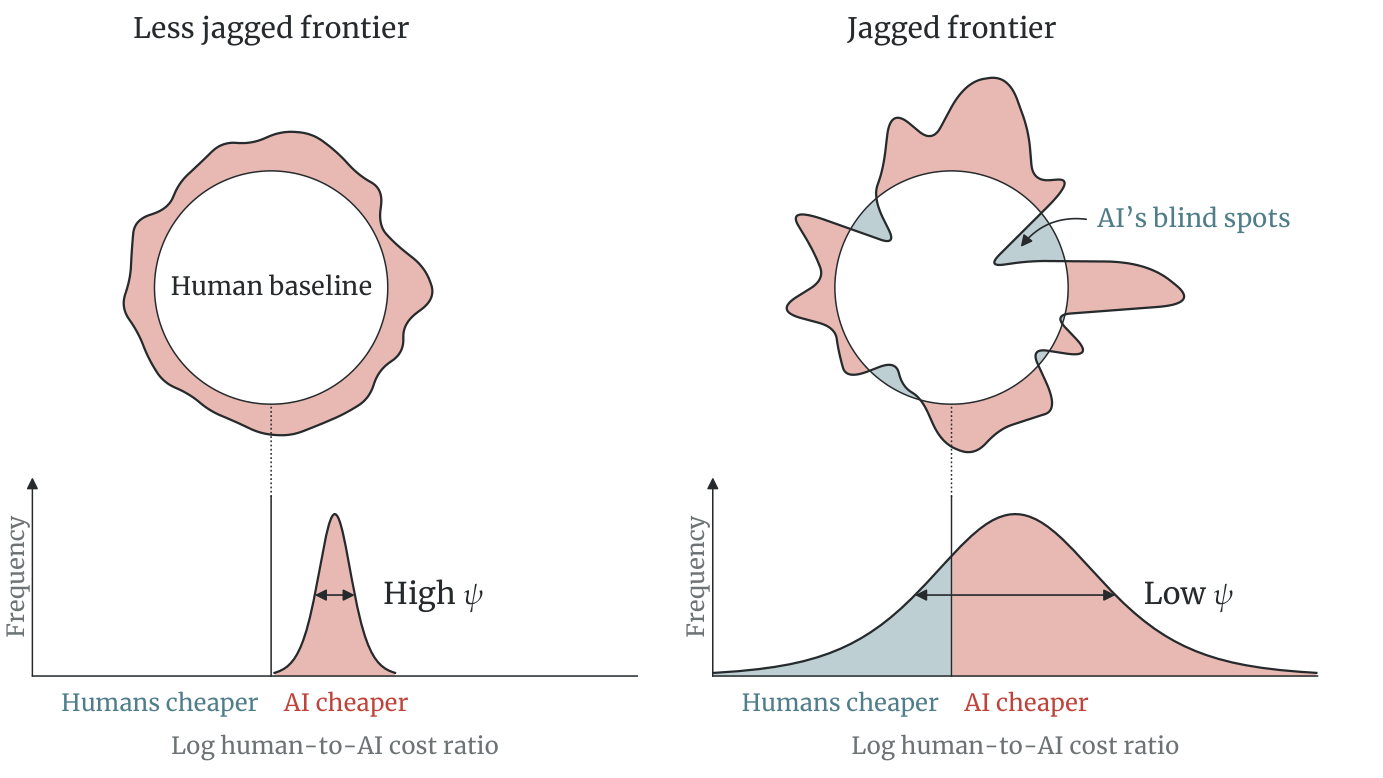
\includegraphics[width=1\textwidth]{jaggedness-figure/output/jaggedness.png}

\vspace{0.25em}
 %
\begin{minipage}[c]{0.94\textwidth}%
{\footnotesize\textit{Notes:}}{\footnotesize{}
The circle is the human baseline, where a task costs the same whether
humans or AI produce it. Each spike of the frontier is one task. Its
distance from the center rises with the task's human-to-AI cost ratio,
so it reaches beyond the circle where AI is cheaper and dips inside
where humans are cheaper. The curves below plot the distribution of
the log human-to-AI cost ratio across tasks, whose spread is proportional
to $1/\psi$. Teal marks AI's blind spots, the tasks where humans
are cheaper.}%
\end{minipage}
\end{figure}


\paragraph{Assignment and equilibrium.}

Task assignment responds to technology and factor prices. Let $\pi_{L,t}$
denote the fraction of tasks produced by workers and let $\pi_{M,t}=1-\pi_{L,t}$
denote the fraction produced by AI. Applying the cutoff rule in \eqref{eq:task-price-main}
to the distribution in \eqref{eq:relative-productivity-cdf} yields
\begin{equation}
\pi_{L,t}=\frac{T_{L}w^{-\psi}_{t}}{T_{L}w^{-\psi}_{t}+T_{M,t}r^{-\psi}_{t}},\qquad\qquad\pi_{M,t}=\frac{T_{M,t}r^{-\psi}_{t}}{T_{L}w^{-\psi}_{t}+T_{M,t}r^{-\psi}_{t}}.\label{eq:assignment-prices}
\end{equation}
The above equation states that a factor performs more tasks when its
technology improves or its price falls.

A competitive equilibrium consists of task quantities, factor allocations,
task prices, a wage, and an AI rental rate such that final good producers
minimize the cost of producing the final output bundle under \eqref{eq:task-aggregator};
each task is assigned to the lower-cost factor per \eqref{eq:task-price-main};
and the aggregate resource constraints \eqref{eq:task-technology-main}
are satisfied. As shown in Appendix \href{https://ahmadlp.github.io/Lashkaripour_AI_Displacement_Online_Appendix.pdf\#page=1}{A},
the conditional distribution of task prices is the same among tasks
produced by workers and by AI. Productivity differences adjust the
extensive margin of assignment, but conditional on assignment the
price of the Human bundle matches that of the AI. Thus, the average
spending per task is the same in both sets, and task shares coincide
with expenditure shares. Market clearing therefore becomes
\begin{equation}
w_{t}L=\pi_{L,t}Y_{t},\qquad r_{t}M_{t}=\pi_{M,t}Y_{t},\label{eq:factor-clearing-main}
\end{equation}
indicating that each factor receives a fraction of the aggregate revenue
proportional to the share of tasks it performs. Combining the assignment
share formula with factor market clearing pins down the relative factor
price as
\begin{equation}
\left[\frac{w_{t}}{r_{t}}\right]^{1+\psi}=\frac{T_{L}}{T_{M,t}}\frac{M_{t}}{L}.\label{eq:relative-factor-price-main}
\end{equation}
Henceforth, let $\widetilde{M}_{t}\equiv[T_{M,t}M^{\psi}_{t}]^{1/(1+\psi)}$
denote the effective AI stock meaning that the supply of AI raises
if either the supply of compute $M_{t}$ increases or the AI frontier
AI techniques $T_{M,t}$ improve through knowledge accumulation. Substituting
the relative factor price back into \eqref{eq:assignment-prices}
gives the task shares directly in terms of technologies and factor
supplies:
\begin{equation}
\pi_{L,t}=\frac{[T_{L}L^{\psi}]^{1/(1+\psi)}}{[T_{L}L^{\psi}]^{1/(1+\psi)}+\widetilde{M}_{t}},\qquad\qquad\pi_{M,t}=\frac{\widetilde{M}_{t}}{[T_{L}L^{\psi}]^{1/(1+\psi)}+\widetilde{M}_{t}}.\label{eq:static-shares}
\end{equation}
It remains to aggregate tasks given the optimal assignment into aggregate
output and price indexes. The derivation is presented in Appendix
\href{https://ahmadlp.github.io/Lashkaripour_AI_Displacement_Online_Appendix.pdf\#page=1}{A} yielding the following representation
for aggregate output as a of productivity fundamentals, 
\begin{equation}
Y_{t}=\gamma^{-1}\left\{ [T_{L}L^{\psi}]^{1/(1+\psi)}+\widetilde{M}_{t}\right\} ^{(1+\psi)/\psi}.\label{eq:aggregate-production}
\end{equation}
where $\gamma>0$ is the a constant composed the parameters related
to the output aggregator and productivity distribution.\footnote{Throughout, we assume that the primitives are positive and finite,
and $\sigma<1+\theta$, so that the price index is finite.} Finally, invoking the labor market clearing condition in \eqref{eq:factor-clearing-main}
yields the following expression for the real wage:
\begin{equation}
w_{t}=\gamma^{-1}\left(\frac{T_{L}}{\pi_{L,t}}\right)^{1/\psi}.\label{eq:acr-wage}
\end{equation}
The real wage measure worker welfare, as the amount of final good
they can purchase with their earnings. Here $\gamma$ and $T_{L}$
are constant primitives. So the only time varying factor that affects
the real wage is $\pi_{L,t}$. And perhaps surpassingly, the real
wage becomes higher the smaller the share of tasks assigned to labor.

\section{Displacement Is Not Immiseration}\label{sec:selection}

The sufficient statistics formula \eqref{eq:acr-wage} uncovers a
surprising relationship between displacement and real wages. It is
best understood by thinking of humans as collectively trading tasks
with a country of AI agents. As labor's task share $\pi_{L,t}$ shrinks,
the gains from trade for labor improve: workers retreat toward a narrower
set of niche tasks, and as a result of specialization, their marginal
productivity grows. Each niche task they produce can be exchanged
for an ever-cheaper, ever-wider range of AI-performed tasks. Somewhat
paradoxically, as the labor share approaches zero, the real wage explodes.

\renewcommand{\thetheorem}{\arabic{theorem}.a}
\def\theHtheorem{\arabic{theorem}.a}

\begin{theorem}[Displacement is not immiseration]\label{thm:selection}
~If AI capabilities are jagged, AI-driven growth raises the real wage
in inverse proportion to labor's share of economic tasks, with elasticity
$1/\psi$, representing the degree of frontier jaggedness:
\[
\Delta\ln w_{t}\ =\ -\frac{1}{\psi}\,\Delta\ln\pi_{L,t}
\]
The labor productivity on human-performed tasks concurrently grows
proportionally with $w_{t}$. And as AI capabilities grow without
bound, labor retreats to a vanishingly small set of tasks; yet its
real wage rises without bound:
\begin{equation}
\pi_{L,t}\to0,\qquad\qquad w_{t}\to\infty\label{eq:selection-limits}
\end{equation}
\end{theorem}

The theorem is proved in Appendix \href{https://ahmadlp.github.io/Lashkaripour_AI_Displacement_Online_Appendix.pdf\#page=13}{B.1}, though
the machinery is pretty simple. As a stock of AI $\widetilde{M}_{t}$
grows, it consumes the share of tasks assigned to labor, given by
\begin{equation}
\pi_{L,t}=\frac{[T_{L}L^{\psi}]^{1/(1+\psi)}}{[T_{L}L^{\psi}]^{1/(1+\psi)}+\widetilde{M}_{t}}\label{eq: Ricardian-assignment}
\end{equation}
And as $\widetilde{M}_{t}$ grows infinitely large, $\pi_{L,t}$ goes
to zero. And the real wage paid to workers grows with the decline
of $\pi_{L,t}$ at an elasticity $1/\psi$.\footnote{The limits in~\eqref{eq:selection-limits} also hold when AI growth
is recursive and reaches a singularity in finite time. If fixed shares
of output finance AI installation and research, AI capabilities diverge
at a finite date; as that date approaches, labor’s task share vanishes
and the real wage rises without bound, at a rate that does not depend
on jaggedness. Appendix~\href{https://ahmadlp.github.io/Lashkaripour_AI_Displacement_Online_Appendix.pdf\#page=24}{B.4} states the result
and Appendix~\href{https://ahmadlp.github.io/Lashkaripour_AI_Displacement_Online_Appendix.pdf\#page=25}{B.5} proves it.} The joint productivity law then makes every percentile of productivity
among the tasks retained by workers a fixed multiple of the real wage.
In other words, worker productivity also explodes. An distinct feature
of the Ricardian assignment model, is that the niche tasks left to
the workers are not \emph{expensive bottlenecks}. To formalize this,
let $s_{L,t}\equiv w_{t}L/Y_{t}$ denote labor's share of GDP. Factor-market
clearing then implies the following.

\begin{corollary}[Task and income shares]\label{cor:task-income-shares}
~At every date, labor's share of GDP equals its share of tasks:
\[
s_{L,t}=\pi_{L,t}.
\]
\end{corollary}

This corollary contrasts with the essential task framework of \citet{jt2026},
where a small set of tasks can command a disproportionately large
cost share. Rather than being driven by such weak links, the explosion
in real wages stems from the unbounded growth in labor productivity
as workers select into niche tasks where AI's relative cost advantage
is less pronounced, precisely the tasks in which human labor retains
a much higher relative cost advantage.

\subsection{Displacement Improves Labor Productivity}

To connect to our result to task-based models of automation like \citep{ar2018},
it is useful to unbundle the real wage effects of AI-driven growth.
Doing so also elucidates why the real wage growth is independent of
the CES production parameter, $\sigma$, which plays a canonical rule
in past studies. Let $\mathcal{H}_{t}$ be the set of tasks workers
perform, of measure $\pi_{L,t}$, and let $\bar{z}_{L,t}$ denote
the average labor productivity on the tasks retained by workers. 
\[
\bar{z}_{L,t}\equiv\left[\int_{i\in\mathcal{H}_{t}}z_{L,t}(i)^{\sigma-1}\right]^{\frac{1}{\sigma-1}}
\]
Each task in $\mathcal{H}_{t}$ costs $w_{t}/z_{L}(i)$ and its demand
is proportional to $Y_{t}p_{t}(i)^{-\sigma}$, so summing revenue
over $\mathcal{H}_{t}$ gives labor's income, $w_{t}L=Y_{t}\,w^{1-\sigma}_{t}\,\pi_{L,t}\,\bar{z}^{\,\sigma-1}_{L,t}$.
Writing in log differences, obtains the following expression for real
wage growth:
\begin{equation}
\Delta\ln w_{t}\ \ =\underbrace{\ \frac{\sigma-1}{\sigma}\,\Delta\ln\bar{z}_{L,t}\ }_{\text{labor productivity on retained tasks}}-\ \underbrace{\ \frac{1}{\sigma}\Delta\ln(1/\pi_{L,t})\ }_{\text{dispalcement}}\ +\ \underbrace{\frac{1}{\sigma}\Delta\ln(Y_{t}/L)}_{\text{aggregate productivity}}.\label{eq:content-decomposition}
\end{equation}
With worker knowledge frontier $T_{L}$ fixed, \eqref{eq:aggregate-production}
makes output per worker proportional to $(1/\pi_{L,t})^{(1+\psi)/\psi}$.
The realized labor productivity $\bar{z}_{L,t}$ is, meanwhile, proportional
to $(1/\pi_{L,t})^{1/\psi}$ because as workers sort into a narrower
range of tasks, their productivity in these task would be greater
than the displaced tasks. Altogether, following the derivation in
Appendix \href{https://ahmadlp.github.io/Lashkaripour_AI_Displacement_Online_Appendix.pdf\#page=9}{A.5}, we get 
\begin{equation}
\Delta\ln(\frac{Y_{t}}{L})=\Big(1+\frac{1}{\psi}\Big)\Delta\ln(1/\pi_{L,t})\qquad\qquad\Delta\ln\bar{z}_{L,t}=\frac{1}{\psi}\,\Delta\ln(1/\pi_{L,t}).\label{eq:productivity-effect}
\end{equation}
Plugging these equations back into Equation \eqref{eq:content-decomposition}
yields our sufficient statistics formula under Theorem~\ref{thm:selection}:
\[
\Delta\ln w_{t}=\frac{1}{\psi}\,\Delta\ln(1/\pi_{L,t}),
\]
The elasticity of substitution, $\sigma$, is absent from this expression
because the extensive and intensive margins of displacement exactly
offset each other. This feature of the model opens the door for measurement
with micro-level data without aggregate production function estimation.

\subsection{General Distribution}

Theorem \ref{thm:selection} invokes the sharp sufficient statistics
formulas implied by the Fréchet distribution. We used Fréchet as the
baseline specification because it is built on a solid theoretical
micro-foundation and emerges organically from new discoveries arriving
according to a Poisson process. The result that displacement is not
immiseration, nonetheless, goes through under a general distribution.
To demonstrate this, suppose that AI progress is Hicks-neutral across
tasks, $z_{M,t}(i)=A_{t}\tilde{z}_{M}(i)$, and let relative productivity
advantage $a(i)\equiv z_{L}(i)/\tilde{z}_{M}(i)$ follow an arbitrary
continuous distribution $G$ that admits a density. The distribution
could be bounded or unbounded and depend on the baseline productivity
$\tilde{z}_{M}$. Ricardian assignment delegates tasks for which $a(i)>a^{*}_{t}$
to workers, where $a^{*}_{t}=A_{t}w_{t}/r_{t}$. Thus, a share $\pi_{L,t}=1-G(a^{*}_{t})$
of tasks are performed by workers in equilibrium. Aggregating tasks
under this assignment profile using the CES price index yields:\footnote{We assume here that $\sigma>1$ and $\Phi(a^{*})$ is finite. For
$\sigma=1$, \[\Phi(a^{*})=\exp\{-\mathbb{E}[\ln\tilde{z}_{M}]+\mathbb{E}[\ln\min\{a^{*}/a,1\}]\}\];
all results below still hold, and $\mathbb{E}[\tilde{z}^{\sigma-1}_{M}]^{1/(\sigma-1)}$
becomes $\exp\{\mathbb{E}[\ln\tilde{z}_{M}]\}$. See Appendix \href{https://ahmadlp.github.io/Lashkaripour_AI_Displacement_Online_Appendix.pdf\#page=15}{B.2}.}
\[
w_{t}=\frac{a^{*}_{t}}{\Phi(a^{*}_{t})},\qquad\qquad\Phi(a^{*})\equiv\mathbb{E}\!\left[\tilde{z}^{\sigma-1}_{M}\min\!\left\{ \frac{a^{*}}{a},1\right\} ^{1-\sigma}\right]^{\frac{1}{1-\sigma}}
\]
The following theorem then follows immediately from the resulting
structure with a formal proof provided in Appendix \href{https://ahmadlp.github.io/Lashkaripour_AI_Displacement_Online_Appendix.pdf\#page=15}{B.2}.

\addtocounter{theorem}{-1}
\renewcommand{\thetheorem}{\arabic{theorem}.b}
\def\theHtheorem{\arabic{theorem}.b}

\begin{theorem}\label{prop:general-displacement}~Suppose the relative
productivity of labor to AI follows a general and potentially bounded
distribution $G$: \begin{enumerate}
\item[(i)] The real wage rises with displacement wherever $G(a^{*})>0$:
\begin{equation}
\frac{\,\mathrm{d}\ln w_{t}}{\,\mathrm{d}\ln(1/\pi_{L,t})}=\frac{s_{M}(a^{*}_{t})}{\eta(a^{*}_{t})}>0,\label{eq:general-elasticity-main}
\end{equation}
where $s_{M}(a^{*})$ is AI's income share and $\eta(a^{*})\equiv-\,\mathrm{d}\ln[1-G(a^{*})]/\,\mathrm{d}\ln a^{*}$
is the tail elasticity of the joint productivity distributoin $G$.

\item[(ii)] Let $\bar{a}<\infty$ denote the upper limit of relative
human productivity. Under standard regularity conditions, unbounded
growth in AI capabilities leads to full displacement, but raises real
wages until it plateaus at a positive but finite rate:
\begin{equation}
\pi_{L,t}\to0,\qquad w_{t}\longrightarrow\bar{a}\cdot\mathbb{E}[\tilde{z}^{\sigma-1}_{M}]^{\frac{1}{\sigma-1}}.\label{eq:general-plateau-main}
\end{equation}
\end{enumerate}
\end{theorem}

\renewcommand{\thetheorem}{\arabic{theorem}}
\def\theHtheorem{\arabic{theorem}}

The theorem states that the real wage rises monotonically to a finite
plateau if $\bar{a}<\infty$ and diverges if the productivity distribution
is unbounded, i.e., $\bar{a}=\infty$. Moreover, if AI has an absolute
advantage in every task in the chosen baseline year, which would be
the case under $\bar{a}=1$, then the real wage converges to AI's
average productivity in that baseline year under explosive AI growth.
More generally, Theorem \ref{prop:general-displacement} states that
the distribution of comparative advantage governs the pace of wage
gains and their eventual limit, but not the direction. The pace in
\eqref{eq:general-elasticity-main} is the ratio of AI's share of
income and the tail elasticity of $G$ (the rate at which displacement
exhausts labor's remaining advantage). The limit, meanwhile, \eqref{eq:general-plateau-main}
depends on the upper endpoint of $G$. If comparative advantage is
bounded, the real wage climbs to a finite plateau rather than collapsing,
even as AI absorbs every task; if it is unbounded, the real wage grows
without bound.\footnote{A constant tail elasticity is not required for the latter: an unbounded
$G$ whose tail elasticity grows without bound still delivers unbounded
growth, though at a lower rate than any power of $1/\pi_{L,t}$---see
Appendix~\href{https://ahmadlp.github.io/Lashkaripour_AI_Displacement_Online_Appendix.pdf\#page=15}{B.2}.} In \citet{ks2024}, a bound on task complexity lets AI automate every
task and the real wage collapses; here, a hard bound on relative advantage
makes the real wage plateau instead, because collapse would require
price of AI services to become exactly zero.\footnote{Fréchet productivity is used because it delivers a closed form, not
because it delivers an optimistic result. Under it the response of
the real wage to displacement in \eqref{eq:general-elasticity-main}
is the constant $1/\psi$, so the real wage is an exact power function
of $1/\pi_{L,t}$ at every task share, while Theorem~\ref{prop:general-displacement}
requires no such assumption. Appendix~\href{https://ahmadlp.github.io/Lashkaripour_AI_Displacement_Online_Appendix.pdf\#page=15}{B.2}
shows that limiting labor's comparative advantage to a finite upper
bound $\bar{a}$ multiplies that response by $1-(a^{*}_{t}/\bar{a})^{\psi}$
at $\sigma=1$, where $a^{*}_{t}$ is the cutoff comparative advantage
at which tasks shift to AI. That factor is close to one while the
cutoff is well below $\bar{a}$ and falls to zero as the cutoff approaches
$\bar{a}$, so a bound makes wage gains smaller rather than larger.}

\subsection{Displacement is Leverage}\label{sec:leverage}

The previous section showed that real wages survive displacement and
even grow without bound as AI capabilities improve. A natural worry
is that the benefits of AI growth diminish as AI takes over more tasks.
Here, we show the opposite: that more displacement amplifies the marginal
wage gains from AI growth. To illustrate this point, let $g_{X}\equiv\dot{X}/X$
denote the growth rate of a generic variable $X$, with $g_{\widetilde{M},t}$
denoting The growth in AI capabilities, $\widetilde{M}_{t}$. When
AI performs a narrow set of tasks, the growth in $\widetilde{M}_{t}$
has little bearing on real wages and consumption. But when AI performs
many tasks, the reduction passes through more broadly to real wages.
In particular, the elasticity of the real wage with respect to the
stock of AI capabilities equals the AI-automated share of tasks over
$\psi$:
\begin{equation}
\frac{\partial\ln w_{t}}{\partial\ln\widetilde{M}_{t}}=\frac{\pi_{M,t}}{\psi}.\label{eq:leverage-elasticity}
\end{equation}
The corresponding wage and output growth rates are
\begin{equation}
g_{w,t}=\frac{\pi_{M,t}}{\psi}g_{\widetilde{M},t},\qquad\qquad g_{Y,t}=\frac{1+\psi}{\psi}\pi_{M,t}g_{\widetilde{M},t}\label{eq:leverage-wage-growth}
\end{equation}
The proof follows from the Ricardian assessment model written in growth
algebra. Ricardian task assignment, per Equation \eqref{eq: Ricardian-assignment},
implies $g_{\pi_{L},t}=-\pi_{M,t}g_{\widetilde{M},t}$, indicating
that AI growth erodes labor's share of tasks in proportion to AI's
current reach. Since the real wage is inversely related to the labor's
task share, $\partial\ln w_{t}/\partial\ln\pi_{L,t}=-1/\psi$, the
two negative effects convert labor displacement from tasks into real
wage growth. The aggregate output equation (\eqref{eq:aggregate-production})
multiplies the real wage growth by $1+\psi$, yielding the growth
division presented above.

An immediate implication of the above result is that faster growth
in AI capabilities raises real wage and output growth in the same
proportion. At a given level of automation $\pi_{M,t}$, doubling
$g_{\widetilde{M},t}$ doubles both growth rates. As AI capabilities
expand further, $\pi_{M,t}$ rises, so subsequent improvements apply
to a larger share GDP and have a larger effect on both wages and output.
Their growth rate nevertheless retains the same ratio $g_{w,t}=\frac{1}{1+\psi}g_{Y,t}.$\footnote{Section \eqref{sec:measurement} estimates $\psi=1.36$,
which implies $1/(1+\psi)\approx0.42$.
Based on these estimates, real wages grow by $0.42$
percent for every $1$ percent increase in output.} This differs from \citet{ks2024}, where automation reduces the number
of tasks reserved for workers, while capital accumulation raises the
productivity of workers who remain. So, wages continue to grow only
if capital accumulation keeps pace with automation and enough tasks
remain exclusive to workers to retain labor scarcity.\footnote{It is important to understand that this result is about the purchasing
power of labor, not its income share. The labor share of income falls
as AI performs more tasks. However, even though workers are stuck
in small pockets of GDP, their wages have high purchasing power because
growth in AI capabilities lowers the cost of performing most tasks,
making consumer goods cheaper.}

\subsection{Task Displacement and Unemployment}\label{sec:unemployment}

Theorem~\ref{thm:selection} shows that the real wage rises as AI
displaces labor from tasks. The result is about the value of labor,
not about jobs: it takes a wage rate that adjusts so that all $L$
workers are employed. This section asks what happens to employment
when the nominal wage cannot fall.

We keep the single sector economy of Section~\ref{sec:model}, with
$L$ workers and AI capacity $M_{t}$, but no longer assign the final
good as the numeraire. Let $P_{t}$ denote the price index of final
output, and write $W_{t}=P_{t}w_{t}$ for the nominal wage rate, $R_{t}=P_{t}r_{t}$
for the nominal rental rate, and $X_{t}=P_{t}Y_{t}$ for nominal GDP.
All $L$ workers are willing to work, but only $N_{t}=e_{t}L$ of
them are employed, where $e_{t}\in(0,1]$ is the employment rate and
$u_{t}=1-e_{t}$ the unemployment rate. In equilibrium the nominal
wage equals the value of the marginal product of labor, and labor's
share of GDP equals its share of tasks as in Corollary~\ref{cor:task-income-shares}.
The factor market clearing condition~\eqref{eq:factor-clearing-main}
becomes
\begin{equation}
W_{t}e_{t}L=\pi_{L,t}X_{t},\qquad X_{t}=W_{t}e_{t}L+R_{t}M_{t},\label{eq:ue-wage-bill}
\end{equation}
where $\pi_{L,t}$ is the share of tasks performed by the $e_{t}L$
employed workers.

With a flexible nominal wage, every worker is employed. Setting $e_{t}=1$
in~\eqref{eq:ue-wage-bill} gives the full employment wage $W^{F}_{t}=\pi_{L,t}(1)X_{t}/L$,
where $\pi_{L,t}(1)$ denotes labor's task share at full employment,
given by~\eqref{eq:static-shares}. As the effective AI stock grows,
$\pi_{L,t}(1)$ falls. At given nominal GDP, the nominal wage must
fall to keep every worker employed, even though the real wage rises
by Theorem~\ref{thm:selection}.

Following \citet{ruv2025}, we suppose that the nominal wage cannot
fall below a floor set by last period's wage, $\underline{W}_{t}=\delta_{w}W_{t-1}$
with $0\leq\delta_{w}\leq1$, and that employment adjusts instead:
\begin{equation}
W_{t}\geq\underline{W}_{t},\qquad0<e_{t}\leq1,\qquad(1-e_{t})(W_{t}-\underline{W}_{t})=0.\label{eq:ue-floor}
\end{equation}
If the full employment wage is below the floor, fewer than $L$ workers
are employed at $W_{t}=\underline{W}_{t}$; if it is at or above the
floor, every worker is employed. The floor applies to all workers,
so the unemployed cannot offer to work for less than the employed,
and unemployment is involuntary. Nominal GDP $X_{t}$ is the nominal
anchor: the model determines real output and the price level, and
$X_{t}$ pins down the nominal scale.

Dividing~\eqref{eq:ue-wage-bill} at date $t$ by the same equation
at date $0$ gives
\begin{equation}
\frac{e_{t}}{e_{0}}=\frac{\pi_{L,t}}{\pi_{L,0}}\times\frac{X_{t}/X_{0}}{W_{t}/W_{0}}.\label{eq:ue-employment}
\end{equation}
When nominal GDP and the nominal wage are unchanged, the last fraction
equals one, and employment falls in proportion to labor's task share:
a one percent decline in labor's task share means a one percent decline
in employment. Employment falls because labor's share of a fixed nominal
GDP falls while the nominal wage cannot, not because each displaced
task is a job.

\begin{proposition}[Task displacement and employment]\label{prop:unemployment}
~Start from full employment, $e_{0}=1$, and let the effective AI stock
$\widetilde{M}_{t}$ grow between dates $0$ and $1$, with $T_{L}$
and $L$ fixed. If nominal GDP is unchanged, $X_{1}=X_{0}$, and the
nominal wage cannot fall, so that~\eqref{eq:ue-floor} holds with
$\delta_{w}=1$, then the unique equilibrium has $W_{1}=W_{0}$ and
\begin{equation}
\frac{e_{1}}{e_{0}}=\frac{\pi_{L,1}}{\pi_{L,0}}<1.\label{eq:ue-prop-employment}
\end{equation}

Let $E_{t}\equiv e_{t}w_{t}$ denote average real earnings per worker,
including the unemployed. The real wage of the employed and average
earnings satisfy
\begin{equation}
\frac{w_{1}}{w_{0}}=\left(\frac{\pi_{L,1}}{\pi_{L,0}}\right)^{-1/\psi},\qquad\frac{E_{1}}{E_{0}}=\left(\frac{\pi_{L,1}}{\pi_{L,0}}\right)^{1-1/\psi}.\label{eq:ue-prop-earnings}
\end{equation}

The real wage rises, but average earnings fall if $\psi>1$, are unchanged
if $\psi=1$, and rise if $\psi<1$.\end{proposition}

The derivation of these results and the proof of the proposition are
in Appendix~\href{https://ahmadlp.github.io/Lashkaripour_AI_Displacement_Online_Appendix.pdf\#page=30}{B.6}. In~\eqref{eq:ue-prop-employment},
$\pi_{L,1}$ is labor's task share in the new equilibrium, with $e_{1}L$
workers employed. It is below the full employment share $\pi_{L,1}(1)$,
because fewer workers perform fewer tasks; using the full employment
share in its place would understate the fall in employment.

Ricardian selection still raises the real wage of the employed, but
under nominal rigidity it does not imply higher average earnings.
Average earnings $E_{t}$ exclude the rental income of AI stock owners
and are not a welfare measure. And full employment returns only through
nominal adjustment, not with time: if, after the shock, the technology
and AI capacity stop changing and nominal GDP grows at a gross rate
$G$, unemployment ends after a finite number of periods when $G>\delta_{w}$
and remains unchanged when $G=\delta_{w}$ (Appendix~\href{https://ahmadlp.github.io/Lashkaripour_AI_Displacement_Online_Appendix.pdf\#page=30}{B.6}).

\section{Jagged Adoption Benefits Workers under Mobility}\label{sec:breadth}

Thus far we have modeled the economy as a single aggregate sector,
which of course overlooks the possibility that AI adoption could be
concentrated in a handful of sectors. Jagged AI adoption across sectors
can have starkly different labor-market consequences than balanced
adoption that affects the entire economy. It turns out that jagged
adoption is, if anything, actually more enriching for workers.The
intuition is straightforward. When AI adoption is concentrated in
certain sectors, it simply creates more room for labor to gain from
comparative advantage, not only across tasks within sectors but also
across sectors themselves.

We formalize this point by extending the baseline model, adding a
finite number of sectors $s\in\{1,\ldots,S\}$. Sector $s$ produces
$Y_{s,t}$ at price $P_{s,t}$ by aggregating over a continuum of
tasks similar to the baseline economy. Labor and AI productivity across
tasks within a sector follow a Fréchet distribution, mirroring the
single sector case. The Fréchet dispersion parameter $\psi>0$ is
the same across sectors, but labor productivity $T_{Ls}$ is sector-specific
and fixed, and stock of AI techniques is also sector-specific $T_{Ms,t}$,
but evolves over time.

We assume no frictions to the mobility of labor and AI agents across
sectors. Sector $s$ uses $L_{s,t}$ units of labor and $M_{s,t}$
units of AI services, with market clearing conditions requiring $\sum_{s}L_{s,t}=L$
and $\sum_{s}M_{s,t}=M_{t}$. The wage rate $w_{t}$ and AI rental
rate $r_{t}$ is equalized across sectors as a result of perfect mobility.
Final demand is a Cobb--Douglas aggregator over sector-level output,
with $\beta_{s}>0$ denoting sector $s$'s expenditure weight, with
$\sum_{s}\beta_{s}=1$. Thus, aggregate output $Y_{t}$ and the unit
price index are given by
\begin{equation}
Y_{t}=\prod^{S}_{s=1}\left(\frac{Y_{s,t}}{\beta_{s}}\right)^{\beta_{s}},\qquad\qquad P_{t}=\prod^{S}_{s=1}P^{\beta_{s}}_{s,t}\equiv1.\label{eq:multisector-final-good}
\end{equation}
Ricardian assignment within each sector implies the following equation
describing the share $\pi_{Ms,t}$ of tasks assigned to AI and the
resulting price index:
\begin{equation}
\pi_{Ms,t}=\frac{T_{Ms,t}(w_{t}/r_{t})^{\psi}}{T_{Ls}+T_{Ms,t}(w_{t}/r_{t})^{\psi}},\qquad P_{s,t}=\gamma_{s}w_{t}\left[T_{Ls}+T_{Ms,t}(w_{t}/r_{t})^{\psi}\right]^{-1/\psi}.\label{eq:sectoral-ai-share}
\end{equation}
where $\gamma_{s}>0$ is fixed price shifter composed of constant
parameters. The fraction $\pi_{Ms,t}$ also represents AI's share
of expenditure in sector $s$, with labor performing the remaining
fraction $1-\pi_{Ms,t}$. Factor market clearing, therefore, pins
down the relative factor price $w_{t}/r_{t}$ as
\begin{equation}
\sum_{s}\beta_{s}\pi_{Ms,t}=\frac{M_{t}}{M_{t}+(w_{t}/r_{t})L}.\label{eq:multisector-clearing}
\end{equation}
The left side represents the share of final expenditure paid to AI
services across all sectors, and the accounting representation of
the AI input cost share. Since $\pi_{Ms,t}$ increases with $w_{t}/r_{t}$
for all $s$, the equation has a unique positive solution. Given that
solution, Cobb--Douglas aggregation and the income accounting identity
$Y_{t}=w_{t}L+r_{t}M_{t}$ yield the following expression for the
real wage:\footnote{The specific details about sectoral employment and AI allocation in
equilibrium are provided in Appendix \href{https://ahmadlp.github.io/Lashkaripour_AI_Displacement_Online_Appendix.pdf\#page=36}{B.7}.}
\begin{equation}
w_{t}=\prod_{s}\left[\gamma^{-\beta_{s}}_{s}\left(\frac{T_{Ls}}{\pi_{Ls,t}}\right)^{\frac{\beta_{s}}{\psi_{s}}}\right].\label{eq:multisector-wage-output}
\end{equation}
Real output is given by $Y_{t}=w_{t}\left(L+\frac{M_{t}}{w_{t}/r_{t}}\right)$.
To compare broad and narrow AI progress, we introduce sectoral heterogeneity
in AI progress as follows: let $A_{t}>0$ be a common AI productivity
index that grows without bound. Sector $s$ follows the power path
\begin{equation}
T_{Ms,t}=T_{Ms,0}A^{\nu_{s}}_{t},\qquad T_{Ms,0}>0.\label{eq:power-paths}
\end{equation}
with the nonnegative exponent $\nu_{s}$ denoting the adoption rate
of sector $s$, the fraction of each advance in the common index that
becomes productive in that sector. At least one sector has a positive
$\nu_{s}$, and those with $\nu_{s}=0$ do not experience any growth
in AI techniques.

This setting is particularly useful for showcasing how AI progress
affects output and wages in different ways. Each sector has a fixed
weight $\beta_{s}$ in aggregate output, so overall output growth
reflects average AI progress across sectors, namely, $\sum_{s}\beta_{s}\nu_{s}$.
Workers, however, sort into sectors where AI improvement is sluggish.
So, progress in those lagging sectors determines how quickly the worker
wages fall relative to AI rental rates. If AI adoption is balanced
across sectors, workers have no lagging sector to retreat to, so real
wages grow less. If AI capacities experience zero growth in at least
one sector, workers retreat to that sector preventing $w_{t}/r_{t}$
from falling further. This pegs the labor share of GDP and causes
real wages to grow at the same rate as output.

\begin{theorem}[Jagged adoption benefits workers]\label{thm:breadth}
~When sector-level AI capabilities grow as $T_{Ms}\propto A^{\nu_{s}}$
with $A\to\infty$, then 
\begin{equation}
\frac{g_{w}}{g_{Y}}\longrightarrow1-\frac{\psi}{1+\psi}\,\frac{\min_{s}\nu_{s}}{\sum_{s}\beta_{s}\nu_{s}}\;\in\;\Big[\frac{1}{1+\psi},\,1\Big].\label{eq:breadth-incidence}
\end{equation}
Labor's income share vanishes if AI advances in every sector ($\nu_{s}>0$
for all $s$) and converges to a strictly positive limit if adoption
is jagged ($\nu_{s}=0$ for some $s$). \end{theorem}

Appendix \href{https://ahmadlp.github.io/Lashkaripour_AI_Displacement_Online_Appendix.pdf\#page=36}{B.7} provides the formal proof for this
theorem. The same logic underpins how employment evolves across sectors.
If AI capabilities advance broadly across all sectors, employment
concentrates in the slowest growing sectors for which $\min_{s}\nu_{s}$.
And if $\min_{s}\nu_{s}=0$, employment in every growing sector converges
to zero. Balanced AI adoption therefore creates an environment where
real wages grow most slowly relative to output.\footnote{The concentrated progress result depends on Cobb--Douglas demand:
with $\sigma_{U}\in(0,1)$, the expenditure shares of sectors with
AI progress fall to zero, $w_{t}/r_{t}$ is pinned down by sectors
with fixed intensity, and $w_{t}$ and $Y_{t}$ approach finite positive
limits, so this result does not determine the limiting ratio of real
wage growth to output growth; Appendix~\href{https://ahmadlp.github.io/Lashkaripour_AI_Displacement_Online_Appendix.pdf\#page=42}{B.8}
gives the equations, proof, and limiting real wage.}

\begin{corollary}[Balanced vs jagged adoption]\label{cor:balanced-progress}
~If labor is perfectly mobile across sectors: Balanced AI adoption
across sectors is the worst-case scenario for labor wage growth. By
contrast, strictly jagged adoption, in which some sectors see no AI
gains at all, lets workers capture most of the growth surplus, with
real wages rising proportionally with output. \end{corollary}

Intuitively, sectors experiencing low AI-driven productivity growth
become relatively expensive, following the same logic as \citeauthor{baumol1967}'s
\citeyearpar{baumol1967} cost disease. Labor concentrates in these
lagging sectors and commands a wage proportional to their price, which
rises relative to the economy-wide price index through rapid AI-driven
growth elsewhere. For these reasons, the real wage $w_{t}$ grows
faster under jagged adoption than under balanced adoption. Importantly,
the unit elasticity of substitution across sectors prevents lagging
sectors from dragging down aggregate growth. But this would not be
the case under complementarity, where the lagging sectors eventually
regulate the aggregate growth rate \citep{ajj2019} and block the
passthrough of AI-driven productivity growth to wages. In the limit
with Leontief aggregation across sectors, jagged adoption is inconsequential.
Insofar as $\min_{s}\nu_{s}\neq0$, we obtain
\[
\frac{g_{w}}{g_{Y}}\longrightarrow\frac{1}{1+\psi},\qquad\qquad\left[\text{Leontief aggregation}\right]
\]
indicating that jagged and balanced adoption have the same effect
on the real wage. It is important to note that the analysis so far
assumes labor moves across sectors without frictions. Under the labor
mobility frictions we explore later, the Baumol effect can erode real
wages for workers stuck in fast-adopting sectors. Their wages are
tied to the price of their own sector's output, which falls in relative
terms due to fast adoption, while lagging sector goods in the consumption
basket become more expensive.

\subsection{Input--Output Linkages}\label{sec:io}

Our analysis so far assumes that humans or agentic AI perform tasks
without using intermediate tools or inputs. Now we introduce a more
realistic model where AI and humans use a Cobb-Douglas bundle of intermediate
inputs from various sectors. Specifically, the primary input has a
weight $\alpha_{s}\in(0,1]$ in production and uses a intermediate
input bundle with share $\Gamma_{ks}$ sourced from sector $k$. The
price of task $i$ per Ricardian assignment is
\[
p_{s,t}(i)=\min\left\{ \frac{w^{\alpha_{s}}_{t}}{z_{Ls}(i)},\frac{r^{\alpha_{s}}_{t}}{z_{Ms,t}(i)}\right\} \times\prod_{k}P^{\Gamma_{ks}}_{k,t}
\]
Let $\lambda_{s}$ be sector $s$'s Domar weight, which is its final
good plus intermediate output relative to GDP, with $\Lambda\equiv\sum_{s}\lambda_{s}$.\footnote{Specifically, $\lambda=(I-\Gamma)^{-1}\beta$ where $\beta_{s}$ denotes
the final expenditure shares. Thus, $\alpha_{s}\lambda_{s}$ represents
the value added share which add up to one.} The share of tasks assigned to AI in equation \eqref{eq:sectoral-ai-share}
is given by
\begin{equation}
\pi_{Ms,t}=\frac{T_{Ms,t}(w_{t}/r_{t})^{\alpha_{s}\psi}}{T_{Ls}+T_{Ms,t}(w_{t}/r_{t})^{\alpha_{s}\psi}},\qquad\pi_{Ls,t}=1-\pi_{Ms,t}.\label{eq:io-ai-share}
\end{equation}
with the elasticity of $\pi_{Ms,t}/\pi_{LS,t}$ \emph{w.r.t.} the
wage-to-rental rate $w_{t}/r_{t}$ given by $\alpha_{s}\psi$ rather
than $\psi$ in the baseline model. The variant of equation \eqref{eq:multisector-clearing}
describes factor market clearing, with the value added shares $\alpha_{s}\lambda_{s}$
in place of $\beta_{s}$, and the aggregate labor share of GDP is
$s_{L,t}=\sum_{s}\alpha_{s}\lambda_{s}\pi_{Ls,t}$, which is a value
added weighted share of tasks done by workers. as shown in Appendix
\href{https://ahmadlp.github.io/Lashkaripour_AI_Displacement_Online_Appendix.pdf\#page=61}{B.11}, the real wage continues to follow a simple
sufficient statistics formula:
\begin{equation}
w_{t}=\prod_{s}\left[\gamma^{-\lambda_{s}}_{s}\left(\frac{T_{Ls}}{\pi_{Ls,t}}\right)^{\frac{\lambda_{s}}{\psi}}\right].\label{eq:io-real-wage}
\end{equation}
This equation differs from the baseline equation \eqref{eq:acr-wage},
in that displacement in sector $s$ contributes to the real wage based
on the Domar weight, $\lambda_{s}$, rather than the final consumption
weight $\beta_{s}$. The fact that $\Lambda=\sum_{s}\lambda_{s}>1$
reflects a larger passthrough from displacement to real wages due
to standard amplification effects through the input-output network.
With $\alpha_{s}=1$ in every sector, the model nests the baseline
model as $\lambda_{s}=\beta_{s}$. Given the constancy of $\gamma_{s}$
and $T_{Ls}$ the change in real wage due to a growth in AI capabilities
at any point in time is
\begin{equation}
\Delta\ln w=-\frac{1}{\psi}\sum_{s}\lambda_{s}\,\Delta\ln\pi_{Ls}.\label{eq:io-real-wage-change}
\end{equation}
Since the weights sum to $\Lambda>1$, an across the board one percent
fall in the share of tasks performed by workers raises the real wage
by $\Lambda/\psi$, which is greater than $1/\psi$ percent implied
by the model that overlooks input-output effects.

A variant of our multi-sector Theorem \ref{thm:breadth} carries over
with minor amendments. Suppose AI capabilities grow following $T_{Ms,t}=T_{Ms,0}A^{\nu_{s}}_{t}$,
all else the same, where $\nu_{s}\geq0$, with strict inequality in
at least one sector. As $A_{t}\to\infty$, the growth in real wage
relative to aggregate output tends to
\begin{equation}
\frac{g_{w}}{g_{Y}}\longrightarrow1-\frac{\psi}{\sum_{s}\lambda_{s}\nu_{s}}\,\min_{s}\left\{ \frac{\nu_{s}}{1+\alpha_{s}\psi}\right\} \;\in\;\Big[\frac{\Lambda}{\Lambda+\psi},\,1\Big].\label{eq:io-incidence}
\end{equation}
Since $\Lambda>1$, the share of output growth appearing as wage growth
under balanced adoption is higher with intermediate inputs than without
them. The lower bound $\Lambda/(\Lambda+\psi)$ is strictly greater
than the bound without input-output loops.\footnote{The worst case scenario is when the adoption rate $\nu_{s}$ is proportional
to $1+\alpha_{s}\psi$. The best case is jagged adoption where $\ensuremath{\min_{s}\{\frac{\nu_{s}}{1+\alpha_{s}\psi}\}=0},$in
which case $\frac{g_{w}}{g_{Y}}\longrightarrow1$. See Appendix \href{https://ahmadlp.github.io/Lashkaripour_AI_Displacement_Online_Appendix.pdf\#page=61}{B.11}
for details.} Two factors contribute to the higher floor. First, input-output loops
amplify the consumer gains from AI-driven growth, which manifests
itself as a fall in the cost of goods relative to the wage rate. Moreover,
as intermediate inputs become cheaper and more productive, the marginal
productivity of labor indirectly benefits from AI-driven growth, putting
upward pressure on wages---a force that is absent in the baseline
model without intermediate input use.\footnote{Our analysis assumes that productivity $z$ is Hicks-neutral. We could
instead model productivity as a shifter specific to each primary factor:
\[p_{s,t}(i)=\min\left\{ (\frac{w_{t}}{z_{Ls}(i)})^{\alpha_{s}},(\frac{r_{t}}{z_{Ms,t}(i)})^{\alpha_{s}}\right\} \times\prod_{k}P^{\Gamma_{ks}}_{k,t}.\]
In this case, intermediate inputs do not influence the task share
assigned to humans versus agentic AI. The share will be still described
by equation \eqref{eq:sectoral-ai-share}. Also, the change in the
real wages will become $\Delta\ln w=-\frac{1}{\psi}\sum_{s}\alpha_{s}\lambda_{s}\,\Delta\ln\pi_{Ls}$.
Since $\sum_{s}\alpha_{s}\lambda_{s}=1$, this case weakens the amplification
effects of input-output linkages. See Appendix \href{https://ahmadlp.github.io/Lashkaripour_AI_Displacement_Online_Appendix.pdf\#page=75}{C.2}
for further details.}

\section{ Universal Wage Growth Can Happen without Mobility}\label{sec:heterogeneity}

A common concern with any rapid technological progress is that workers
may not be able to adapt because of frictions to labor mobility across
sectors. This section argues that the welfare gains from AI growth
can materialize despite high frictions to labor mobility across sectors.
This is precisely what separates AI growth from other technological
shocks like trade openness. To show this, extend our multi-sector
model to allow for multiple groups of workers that sort into sectors
based on their potential earnings \`a la  Roy \citep{cv2015,gry2023}.
To this end, partition workers into groups indexed by $g$, each with
population mass $\bar{L}_{g}>0$. Because labor mobility is subject
to frictions across sectors, each sector pays a wage $w_{s,t}$ per
efficiency unit of labor. An individual's wage income is if working
in sector $s$ is $w_{s,t}z_{s}$, where $z_{s}$ is their efficiency
drawn the group-level multivariate Fréchet distribution
\[
F_{g}(\mathbf{z})=\exp\!\left(-\sum_{s}a_{gs}z^{-\kappa_{g}}_{s}\right),\qquad\kappa_{g}>1,
\]
The parameter $a_{gs}\geq0$ represents the group $g$'s overall productivity
to sector $s$, and $\kappa_{g}$ governs the dispersion in worker
productivity across sectors. $\kappa$ therefore reflects frictions
to labor mobility, Because more dispersion means that workers cannot
easily move sectors because they are unlike to command the same income
in a different sector.\footnote{We do not assume that every education group can work in every sector.
Instead we impose that for every group $g$, there is at least one
sector for which $a_{gk}>0$ , and that every sector has positive
employment in the baseline equilibrium.} The Fréchet structure yields closed-form expressions for group-level
earnings and employment shares across sectors. Namely, the share of
group $g$ workers employed in sector $s$ and the group's average
earnings are
\[
\mu_{gs,t}=\frac{a_{gs}w^{\kappa_{g}}_{s,t}}{\sum_{k}a_{gk}w^{\kappa_{g}}_{k,t}},\qquad\qquad W_{g,t}=\Gamma\!\left(1-\frac{1}{\kappa_{g}}\right)\left(\sum_{s}a_{gs}w^{\kappa_{g}}_{s,t}\right)^{1/\kappa_{g}}.
\]
The group's average real income is thus $W_{g,t}$. A larger $a_{gs}$
draws more workers from group $g$ to sector $s$ at a given wage
vector and a larger $w_{s,t}$ draws workers from all groups who can
feasibly work in that sector. Labor-market clearing equates the supply
and demand for labor in sector $s$
\[
w_{s,t}\ell_{s,t}=\sum_{g}\bar{L}_{g}\mu_{gs,t}W_{g,t}=\beta_{s}\pi_{Ls,t}Y_{t},
\]
with $\ell_{s,t}$ denoting equilibrium employment in efficiency units
in that sector and $\pi_{Ls,t}$ is the share of tasks assigned to
labor in that sector:
\[
\ensuremath{\pi_{Ls,t}=\frac{T_{Ls}}{T_{Ls}+T_{Ms,t}(w_{s,t}/r_{t})^{\psi}},}
\]
Here, $\kappa_{g}$ governs mobility across sectors, and labor becomes
frozen in their respective sectors in the limiting case where $\kappa\downarrow1$,
representing what is considered a \emph{specific factors economy}.
As before, $\psi>0$ governs comparative advantage between workers
and AI within sectors. The real income of workers in group $g$:
\[
\begin{aligned}W_{g,t} & =\Gamma\left(1-\frac{1}{\kappa_{g}}\right)Y_{t}\left[\sum_{s}a_{gs}\left(\frac{\beta_{s}\pi_{Ls,t}}{\ell_{s,t}}\right)^{\kappa_{g}}\right]^{1/\kappa_{g}},\\
Y_{t} & =\prod_{s}\left[\Phi_{s}\ell_{s,t}\pi^{-\frac{1+\psi}{\psi}}_{Ls,t}\right]^{\beta_{s}}.
\end{aligned}
\]
where $\Phi_{k}\equiv T^{\frac{1}{\psi}}_{Lk}/\gamma_{k}\beta_{k}$
is a sector-level constant. AI capability grows according to $T_{Ms,t}=T_{Ms,0}A^{\nu_{s}}_{t},$,
with $\nu_{s}\geq0$ and positive average progress: $\sum_{s}\beta_{s}\nu_{s}>0$.
An interesting special case emerges when labor is frozen to a given
sector: $\left.\hat{\ell}_{s}\right|_{\kappa\downarrow1}=1$. In this
case, the percent change in real wages from growing AI capabilities
can be expressed as
\[
\left.\Delta\ln w_{s}\right|_{\kappa\downarrow1}\ =\ \left.\Delta\ln\pi_{Ls}\ -\ \frac{1+\psi}{\psi}\sum_{s'}\beta_{s'}\Delta\ln\pi_{Ls'}\,\right|_{\kappa\downarrow1}.
\]
The first term captures the downward pressure on wages as AI performs
more tasks in sector $s$, with better capabilities. The second term
captures the increase in purchasing power through aggregate productivity
growth. Greater AI capabilities raise aggregate output across all
sectors, raising the purchasing power of wages. Appendix \href{https://ahmadlp.github.io/Lashkaripour_AI_Displacement_Online_Appendix.pdf\#page=47}{B.9}
establishes a real wage floor per sector: there is a constant $c_{s}>0$,
independent of $A_{t}$, such that $w_{s,t}\geq c_{s}A^{\frac{1}{\psi}\sum_{k}(\beta_{k}\nu_{k})-\frac{\nu_{s}}{1+\psi}}_{t}$.
Moreover, even when frictions to labor mobility across sectors are
prohibitive then the elasticity of real wage w.r.t. AI productivity
growth is
\[
\left.\frac{\mathrm{d}\ln w_{s,t}}{\mathrm{d}\ln A_{t}}\right|_{\kappa\downarrow1}\longrightarrow\frac{1}{\psi}\sum_{k}\beta_{k}\nu_{k}-\frac{\nu_{s}}{1+\psi}.
\]
Thus unless AI adoption is extremely jagged across industries, real
wages benefit from AI growth across the board even when workers cannot
switch sectors. The following proposition formalizes this result in
terms of growth calculus.

\begin{sectiontheorem}[Wage divergence]\label{thm:wage-divergence}
~As AI capabilities grow, $A_{t}\to\infty$, a worker employable only
in sector $s$ receives the following share of output growth:
\[
\left.\frac{g_{w_{s}}}{g_{Y}}\right|_{\kappa\downarrow1}\longrightarrow1-\frac{\psi}{1+\psi}\frac{\nu_{s}}{\sum_{k}\beta_{k}\nu_{k}}
\]
 And regardless of workers' profiles and their mobility across sectors,\footnote{Under the strict reverse inequality, the real wage of a worker employable
only in the sector with the fastest AI adoption falls to zero.}
\[
\frac{\max_{s}\nu_{s}}{\sum_{k}\beta_{k}\nu_{k}}<\frac{1+\psi}{\psi}\qquad\Longrightarrow\qquad\text{every worker's real wage grows without bound}
\]
\end{sectiontheorem}

The flip side of the above result is that if $\frac{\max_{s}\nu_{s}}{\sum_{k}\beta_{k}\nu_{k}}>\frac{1+\psi}{\psi}$,
AI adoption is so much faster in one sector than the rest of the economy
that a worker who cannot leave that sector eventually sees their real
earning power approach zero. The reason is that jagged adoption will
produce a Baumol's cost disease effect. Sectors that are slow to adopt
will become increasingly expensive relative to fast-adopting sectors.
So, workers in fast-adopting sectors will see the purchasing power
of their wage fall w.r.t. the consumer goods purchased from lagging
sectors. That being said, the condition in Theorem \ref{thm:wage-divergence}
is satisfied based on our forthcoming estimation. The left-hand side
is $(\max_{s}\nu_{s})/\sum_{k}(\beta_{k}\nu_{k})\leq1.63$
in every year of our counterfactual, compared with $(1+\psi)/\psi=1.74$.
So, in this simple setting, even a worker stuck in the sector experiencing
the fastest AI adoption will see their real wage grow at no less than
$6.06$ percent of the rate of output
growth.\footnote{The result holds in a weaker form in an economy where production involves
fixed or slowly growing sector-specific capital like machinery. In
that case, increased demand raises the cost of capital intensive goods.
This limits the gain in the purchasing power of wages and can lower
the real wages of workers in some sectors even when the condition
in Theorem \ref{thm:wage-divergence} holds. Appendix \href{https://ahmadlp.github.io/Lashkaripour_AI_Displacement_Online_Appendix.pdf\#page=91}{C.9}
derives the formula describing real wage growth under fixed capital.}

\subsection{The Jevons Paradox}\label{sec:jevons}

We close this section with a remark on the Jevons paradox, the idea
that agentic AI growth can make cognitive tasks so productive that
the resulting demand boost for knowledge work outweighs the displacement
effect, raising knowledge workers' wages relative to the rest of the
economy \citep{jevons1865}. Under this logic, the same knowledge
workers that AI displaces are those who gain most from AI-driven growth.
To explore this phenomenon, we must look beyond the baseline Cobb--Douglas
aggregator across sectors, since inter-sectoral substitution is the
main driver of the paradox. We consider the simplest alternative,
which is a CES utility aggregator across sectors with elasticity $\eta>0$.
Keeping everything else unchanged in the model, sector $s$'s share
of final expenditure is
\begin{equation}
\omega_{s}\equiv\frac{P_{s}Y_{s}}{Y}=\frac{\beta_{s}P^{1-\eta}_{s}}{\sum_{k}\beta_{k}P^{1-\eta}_{k}},\label{eq:jevons-share}
\end{equation}
The wage bill in sector $s$ becomes $w_{s}L_{s}=\pi_{Ls}\omega_{s}Y$.
With an endogenous sector-level expenditure share $\omega_{s}$, the
response of wages in sector $s$ to rapid AI-driven growth is regulated
by two effects. First, substitution effects, whereby AI progress in
sector $s$ lowers the task share of labor $\pi_{Ls}$ with elasticity
$\psi$. Second, income effects, where AI-driven growth makes the
sector more productive, deflating $P_{k}$ and increasing the sector-level
expenditure share $\omega_{s}$ with elasticity $\eta-1$. The income
effect will dominate the substitution effect if and only if $\eta>1+\psi$,
increasing the wage bill with AI-driven growth.\footnote{This is the Hicks rule of derived demand \citep{hicks1932}, the condition
in \citet{ar2018} for the productivity effect to dominate displacement.
The running assumption in all cases is that a sector is small enough
that $Y$ and $r$ are unaffected.} In the limit $\kappa\downarrow1$, where labor is immobile across
sectors, the relative wage across any two sectors is fully determined
by the relative displacement effect as\footnote{See appendix \href{https://ahmadlp.github.io/Lashkaripour_AI_Displacement_Online_Appendix.pdf\#page=57}{B.10} for the derivation.}
\begin{equation}
\frac{\hat{w}_{s}}{\hat{w}_{k}}=\left(\frac{\hat{\pi}_{Lk}}{\hat{\pi}_{Ls}}\right)^{\frac{\eta-1-\psi}{\eta\psi}},\label{eq:jevons-ratio}
\end{equation}
If the inter-sectoral substitution elasticity is $\eta=1+\psi$, the
income effect exactly offsets the substitution effects, laving relative
wages unaffected. This invariance holds irrespective of the mobility
paramater $\kappa_{g}$. When $1<\eta<1+\psi$, substitution effects
dominate and there is no paradox, as wages drop more in knowledge-intensive
sectors where agentic AI growth causes more displacement. However,
if the inter-sectoral substitution elasticity $\eta>1+\psi$ is sufficiently
large, the income effect dominates the substitution effect, elevating
wages in sectors where AI displacement is highest.

\section{ AI versus other Labor-Saving Technologies}\label{sec:ai-versus-trade}

\subsection*{AI \emph{versus} Engines}

A common example widely used to caution against the effects of AI-driven
displacement is the fate of horses. At the beginning of the 20th century,
engines displaced horses, rendering them economically irrelevant and
unraveling a rapid decline in the horse population. Many worry that
what engines did to horses, agentic AI will do to humans. Our framework
points to an important distinction between horses and humans. What
made horses especially vulnerable to full displacement and immiserization
is that their productivity profile was very similar to engines Across
manual tasks . From the lens of our Ricardian assignment model, this
corresponds to $\rho=1$, which implies An infinitely large Ricardian
dispersion parameter, i.e., $\psi\rightarrow\infty$. Going back to
our sufficient statistics formula, $\Delta\ln w=-\frac{1}{\psi}\Delta\ln\pi_{L}$,
the immediate implication of this is that real wages would not grow
with displacement, $\Delta\ln w=0$.\footnote{The collapse in the horse population also requires that the cost of
keeping horses exceeded their income.}What makes humans different from horses, potentially, is that They
perform a much wider range of tasks. They are adaptable, and their
productivity profile is different from agentic AI. Even if AI performs
every task better than humans, the relative difference between humans
and agentic AI across tasks is not uniform.

\subsection*{AI \emph{versus} Trade}

Trade is often invoked as an example of a large-scale technological
change that led to massive displacement. It immiserated workers in
import-competing sectors, and makes one wonder why AI-driven displacement
would be any different? Theorem \ref{thm:wage-divergence} sheds light
on this exact question. It states that when sector $s$ undergoes
a technological change and workers cannot leave that sector, their
real wage prospects depend on the concentration of the shock in that
sector, $\nu_{s}/\bar{\nu}$, and the Ricardian dispersion parameter,
$\psi$. Their real wage goes down iff $\nu_{s}/\bar{\nu}>(1+\psi)/\psi$.
The trade shock wad characterized by $\nu_{s}=1$ in trade-exposed
manufacturing sectors $\mathscr{T}$ and $\nu_{s}=0$ elsewhere. This
lead to a high concentration index $\nu_{s}/\bar{\nu}=1/\beta_{\mathscr{T}}$
for manufacturing sectors, where $\beta_{\mathscr{T}}=\sum_{s\in\mathscr{T}}\beta_{s}$
is the share of manufacturing in GDP.

The trade shock would have benefited workers through Ricardian assignment
iff $\psi<\frac{\beta_{\mathscr{T}}}{1-\beta_{\mathscr{T}}}$, but
this condition was far from satisfied. Data from 2000 points to $\beta_{\mathscr{T}}\approx0.15$
for the US economy, while the dispersion parameter in an international
trade context is often estimated to be around four.\footnote{Compare this with agentic AI adoption which is spread more equally
across all sectors of the economy. Our forthcoming analysis shows
that $\max_{s}\nu_{s}/\bar{\nu}=1.63$, which is
well below $\nu_{s}/\bar{\nu}=1/\beta_{\mathscr{T}}\approx6.7$.} Thus, the conditions were stacked against workers in the manufacturing
sector as the concentration and trade elasticity far exceeded the
values needed for real wag insulation despite displacement. Intuitively,
the manufacturing workers' job prospects were heavily influenced by
import competition, whereas the other sectors were insulated and did
not experience significant productivity gains. Thus, nominal manufacturing
wages declined, while the CPI, or consumer price index, did not budge
much and even rose because of the higher price of non-traded services.

The fact that international trade in tasks is concentrated in select
industries and operates under a high trade elasticity is a natural
consequence of high inter-country trade costs. Some sectors are intrinsically
not amenable to cross-country trade. So, the trade shock will be concentrated
in internationally traded sectors. For the same reasons, if producing
goods requires performing a sequence of tasks, it is extremely costly
to perform those tasks in different locations. Trade will generally
involve performing a bundle of consecutive tasks in one location to
minimize intermediate border crossing. To formalize this point, suppose
tasks in sector $s$ are grouped in blocks of $k_{s}$ consecutive
tasks.\footnote{We take blocks as given here. They emerge when tasks are performed
in sequence and an intermediate good that changes country between
two consecutive tasks requires $f\ge0$ units of border crossing services,
produced with home and foreign labor in Cobb--Douglas shares of one-half
each. The country of each task is then chosen to minimize the cost
of performing tasks plus the cost of border crossing, and a block
is a full run of consecutive tasks in one country.} Instead of assigning countries to individual tasks, countries are
assigned to blocks of tasks, with each block produced by the country
that has lowest cost. As shown in Figure \ref{fig:task-bundling-jaggedness},
the bundling of tasks attenuates the effective jaggedness of trade
as a labor-saving technology. As a result, trade leaves fewer Ricardian
crevasses for the workers to select into. Appendix \href{https://ahmadlp.github.io/Lashkaripour_AI_Displacement_Online_Appendix.pdf\#page=69}{B.12}
formalizes this point and the implications for wage growth are immediate
from Theorem \ref{thm:breadth} and \ref{thm:wage-divergence}. If
labor is immobile, in the limit as foreign's relative productivity
in sector $s$ grows without bound, a home worker employed in that
sector receives a real wage growth characterized by
\begin{equation}
\frac{g_{w_{s}}}{g_{Y}}\longrightarrow1-\frac{k_{s}\psi}{1+k_{s}\psi}\,\frac{\nu_{s}}{\sum_{s'}\beta_{s'}\nu_{s'}}.\label{eq:unit-of-reassignment}
\end{equation}
The worker's real wage rises without bound if $\nu_{s}/\sum_{s'}\beta_{s'}\nu_{s'}<1+1/k_{s}\psi$
and falls to zero under the strict reverse inequality. With $k_{s}=1$
in every sector, \eqref{eq:unit-of-reassignment} reduces to the specific
factor case of Theorem \ref{thm:wage-divergence}. The product $k_{s}\psi$
is the trade elasticity in the limit where foreign technological advantage
in sector $s$ grows without bound.

\begin{figure}[t]
\centering\caption{Task bundling and effective jaggedness}\label{fig:task-bundling-jaggedness}
\vspace{0.25em}
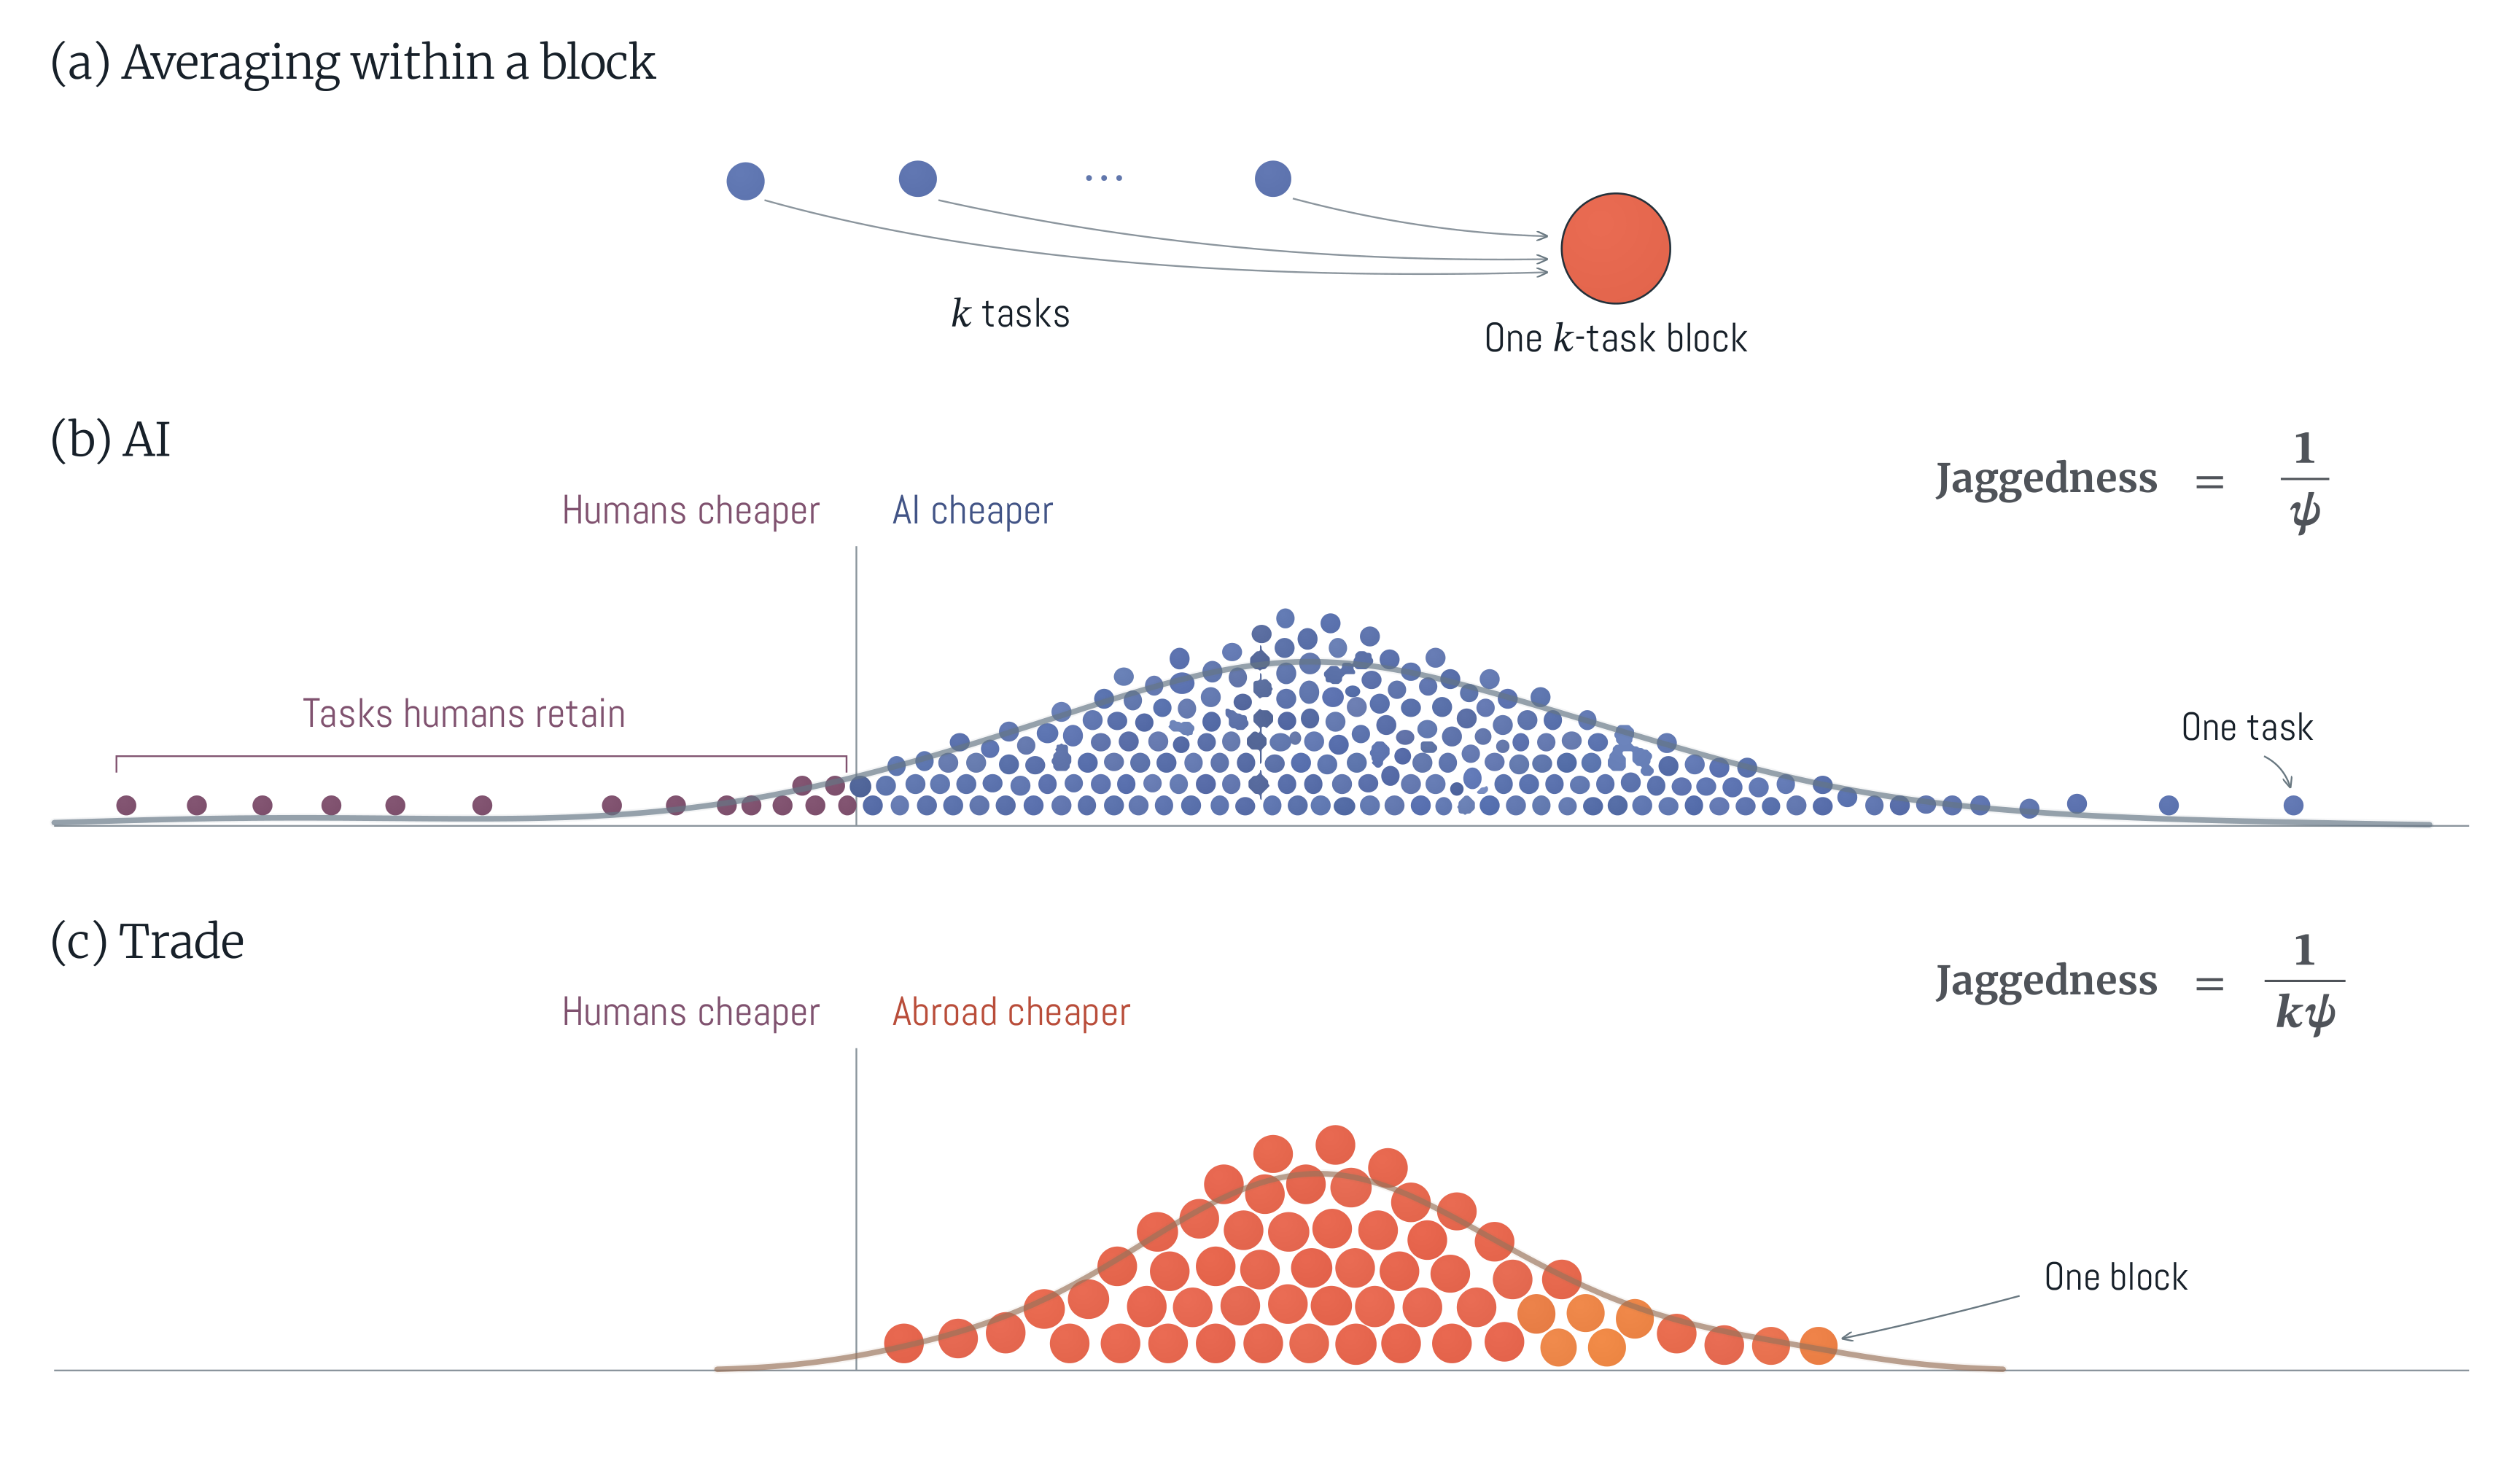
\includegraphics[width=1\textwidth]{task-bundling-figure/output/task-bundling.png}
\end{figure}


\section{Mapping Model to Data}\label{sec:measurement}

This section estimates $\psi$, the parameter that reflects the jaggedness
of AI frontier and regulates the strength of Ricardian comparative
advantage. I use two methods for estimating $\psi$. The first method
recover $\psi$ from the share $\pi_{M}$ of tasks that AI can complete
below human cost and the median cost gap between AI and humans. The
second method identifies $\psi$ from the curvature of the relative
cost distribution. Both methods require data moments that are currently
available only for software engineering (SWE) tasks. The reason is
that software tasks have largely observable contexts and verifiable
outputs, making them amenable to automation and benchmarking.

A natural question is whether the value of $\psi$ estimated from
software engineering tasks is representative of the broader economy.
I view these estimates as a plausible upper bound on the economy-wide
$\psi$. The argument is that the same features that make software
tasks amenable to AI automation are also likely to make AI productivity
relatively uniform across tasks. The performance of AI would be arguably
more varied across tasks that combine text-based and embodied elements.
Take, for instance, tasks related to legal work, which range from
drafting documents to appearing in court. The former is a standard
AI task, but the latter is more difficult for AI to perfect. Extrapolating
from this example, one could argue that AI's productivity is likely
to be more dispersed across tasks outside software engineering.

This interpretation makes our quantitative results that follow conservative,
considering the paper's central premise. The paper argues that AI-driven
growth can raise workers' real wages despite large-scale displacement.
Using the software-based estimate for $\psi$ would understate the
real-wage gains generated by Ricardian selection, because a larger
$\psi$ implies less scope for comparative advantage across tasks.\footnote{The parameter $\psi$ also sets the size of the implied improvement
in AI capabilities given an observed average cost decline. So, a lower
$\psi$ makes the counterfactual shock smaller. Appendix \href{https://ahmadlp.github.io/Lashkaripour_AI_Displacement_Online_Appendix.pdf\#page=104}{D.3}
runs the model using lower estimates for $\psi$ and shows larger
gains in real wages but smaller gains in real output.}

\paragraph{Data.}

Our estimation uses data from 484 software-engineering drawn
from 12 open-source repositories in SWE-bench Verified
\citep{jimenez2024,openai2024verified}. The panel records 32
AI system configurations released from 2024 through
2026 and evaluated by Epoch AI, an independent research
organization \citep{epoch2026}. The 32 configurations
arrive on 26 distinct release dates, which is also
the time dimension used throughout the paper. AI cost is the API charge
for the tokens used in a successful attempt, scaled by a factor of
175 that stands for deployment costs beyond tokens
(Appendix \href{https://ahmadlp.github.io/Lashkaripour_AI_Displacement_Online_Appendix.pdf\#page=101}{D.1}). Human cost is based on a
professional assessment of the time needed to complete the same task,
multiplied by one of three hourly wage rates: the BLS mean software
developer wage, an effective BLS wage scaled up by a fixed multiplier
1.4 to cover benefits and overhead, and a
freelance rate of 100 dollars per hour \citep{bls2024oews,bls2023ecec,upwork2026}.
All costs are converted to July~2026 dollars using the CPI-U
deflator \citep{bls2026cpi}. Our baseline analysis constructs relative
cost ratios using effective labor wages, adjusted for overhead. Since
the experts report a range of hours rather than a single number for
human time requirements, we use the midpoint of that range and treat
tasks marked as \textquotedbl more than four hours\textquotedbl{}
to never exceed 16 hours. AI cost is calculated based
on the cheapest rate available from any model that completed the task
by June~2026. Appendix \href{https://ahmadlp.github.io/Lashkaripour_AI_Displacement_Online_Appendix.pdf\#page=101}{D.1}
provides further details on the construction and provenance.

\subsection{Estimating the Jaggedness of the AI Frontier ($1/\psi$)}

The model lets us estimate $\psi$ by comparing worker and AI costs
task by task. Recall that the unit cost of producing task $i$ is
$c_{L}(i)=w/z_{L}(i)$ workersI and $c_{M}(i)=r/z_{M}(i)$ with AI.
Denote the spread between the human and AI cost as
\begin{equation}
D(i)\equiv\frac{c_{L}(i)}{c_{M}(i)}=\frac{w}{r}\frac{z_{M}(i)}{z_{L}(i)}.\label{eq:measured-cost-advantage}
\end{equation}
such that $D(i)>1$ indicates that AI can complete the task more cheaply
than human. It is straightforward to show that for any where $d\in\mathds{R}_{+}$,
the nested-Fréchet productivity distribution implies
\begin{equation}
\Pr[D(i)\leq d]=\left[1+\Omega d^{-\psi}\right]^{-1},\qquad\qquad\Omega\equiv\frac{T_{M}}{T_{L}}\left(\frac{w}{r}\right)^{\psi}.\label{eq:measurement-cost-advantage-cdf}
\end{equation}
The share of assignments for which agentic AI is cheaper than humans
is therefore $\pi_{M}=\Pr[D(i)>1]$. Below I use the above expression
to develop two methods for estimating $\psi$ using data on SWE tasks.

\paragraph{Release-Level Regression.}

Let $m\equiv\operatorname{Med}[D(i)\mid D(i)>1]$ denote the median
cost spread between humans and AI among tasks that AI performs cheaper.
At cost parity, where $d=1$, equation \eqref{eq:measurement-cost-advantage-cdf}
gives $\Omega=\pi_{M}/(1-\pi_{M})$. Since $m$ divides the tasks
above cost parity in half, it follows that $\Pr[D(i)\leq m]=1-\pi_{M}/2$.
Plugging these values back into Equation gives
\begin{equation}
m^{\psi}=\frac{2-\pi_{M}}{1-\pi_{M}}\label{eq:measurement-mapping}
\end{equation}
If the productivity distribution follows a nested-Fréchet, Equation
\eqref{eq:measurement-mapping} holds at every release date with the
same $\psi$. This equation will forms the basis of our first estimation
method. Let $\widehat{\pi}_{M,t}$ denote the sample share of tasks
completed by AI below human cost by date $t$, and let $\widehat{m}_{t}$
denote the corresponding conditional median.\footnote{To harmonize the sample across both methods, the tasks with the greatest
AI cost advantage must be left out for every released date. However,
$\widehat{m}_{t}$ is nearly unchanged without these tasks.} Rearranging equation \eqref{eq:measurement-mapping} and taking logs
gives the estimating equation across release dates:
\begin{equation}
\ln\frac{2-\widehat{\pi}_{M,t}}{1-\widehat{\pi}_{M,t}}=\psi\ln\widehat{m}_{t}+\varepsilon_{t},\label{eq:sm-regression}
\end{equation}
$\varepsilon_{t}$ denotes measurement error associated with hourly
human cost assessment across in release date $t$. For inference,
I bootstrap by repository: standard errors are calculated by selecting
12 repositories at random \emph{with replacement}
and recomputing the shares, the medians, and $\widehat{\psi}$.

\paragraph{Task-level regression.}

The previous regression uses only two values of $d$ per release date:
cost parity, $d=1$, and median, $d=m_{t}$. The next method, leverages
the full distribution of the cost spread $D(i)$ across tasks. Following
equation \eqref{eq:measurement-cost-advantage-cdf}, the share of
tasks with cost spread above $d$, relative to the share below $d$,
equals $\Omega d^{-\psi}$. Let $S_{t}(d)\equiv\Pr[D(i)>d]$ denote
the share of tasks whose cost spread exceeds $d$ at release date
$t$. Then
\[
\ln\frac{S_{t}(d)}{1-S_{t}(d)}=\ln\Omega_{t}-\psi\ln d.
\]
The left-hand side represents the log odds ratio that a task has a
cost spread above $d$. Thus $\psi$ is the constant elasticity at
which the log odds ratio falls with $\ln d$. The intercept $\ln\Omega_{t}=\ln[\pi_{M,t}/(1-\pi_{M,t})]$
is pinned down by $\pi_{M,t}$, which is directly observable. Plugging
the expression for $\ln\Omega_{t}$ back into the above equation obtains
our estimating equation 
\begin{equation}
\ln\frac{\widehat{S}_{i,t}}{1-\widehat{S}_{i,t}}-\ln\frac{\widehat{\pi}_{M,t}}{1-\widehat{\pi}_{M,t}}=-\psi\ln d_{i,t}+\varepsilon_{i,t}.\label{eq:task-regression}
\end{equation}
Here $d_{i,t}$ is the cost spread of task $i$ at date $t$, and
$\widehat{S}_{i,t}$ is the share of the 484 tasks whose
cost spread exceeds $d_{i,t}$. To harmonize the sample across methods
we restrict the sample to tasks where $d\geq1$ and drop the task
with the largest cost spread, for which $\widehat{S}_{i,t}=0$. by
construction. Lastly, to limit the influence of outliers, I winsorize
the sample of cost spreads at the 5\% level.

\subsection{Estimation Results}

Table~\ref{tab:two-estimates} reports the estimated $\psi$ under
both methods. The release-level regression yields $\widehat{\psi}=1.14$,
and task-level regression delivers $\widehat{\psi}=1.36$,
both with narrow bootstrapped standard error bands.\footnote{The small bootstrapped standard errors capture only the random draw
of repositories and not measurement error in human costs. Each draw
changes which repositories are in the sample but keeps the assessed
completion times and human cost conventions fixed. Appendix \href{https://ahmadlp.github.io/Lashkaripour_AI_Displacement_Online_Appendix.pdf\#page=104}{D.3}
shows how much the estimate changes across human cost specifications
and wage bases.} Figure \ref{fig:price-of-automation} reports the mechanics of each
estimation strategy. Panel (a) shows the path of $\pi_{M}$ over release
dates, showing that the share of tasks AI completes below human cost
increased to 75.2 percent by the end of
the sample.\footnote{A simple regression of AI cost on release date gives an annual coefficient
of -1.57, which implies a 79.2
percent decline per year.} Panel (b) plots the distribution of the human-to-AI cost ratio $G(.)$
among tasks dominated by AI at the latest release. For the median
such task, the human costs 4 times
more than agentic AI. The release-level regression identifies $\psi$
from these two data moments across the 26 release
dates. Panel (c) plots the log odds ratio against the cost spread
across all tasks. The slope of the fitted line corresponds to the
$\psi$ identified by the task-level estimation. Both methods, deliver
comparable results which is encouraging.

\paragraph{Robustness.}

A range of robustness checks is reported in the appendix. Specifically,
I re-run the estimations under several alternative configurations.
First, I re-run the task-level estimation on the full sample without
winsorization, which leaves the estimated $\psi$ mostly unchanged
at 1.35. I also experiment with various
proxies for the hourly wage drawn from different sources. Changing
the hourly wage shifts the relative human-to-AI cost, potentially
affecting the release-level regression that depends on the sample
median cost. The estimated $\psi$ stays between 0.99
and 1.95 under all explored specifications. Appendix
Figure \href{https://ahmadlp.github.io/Lashkaripour_AI_Displacement_Online_Appendix.pdf\#page=105}{B1} reports the full session sensitivity
grid. The takeaway is that the estimated $\psi$ remains in a range
of values that all predict qualitatively the same real-wage and displacement
trajectory when inserted into the model.

\begin{table}[t]
\centering  \caption{Estimation results: Productivity Dispersion Parameter $\psi$}
\label{tab:two-estimates} \begin{tabular}{l d{2.4} d{2.4}}
\toprule
 & \multicolumn{1}{c}{Release level} & \multicolumn{1}{c}{Task level} \\
 & \multicolumn{1}{c}{(1)} & \multicolumn{1}{c}{(2)} \\
\midrule
Dispersion parameter $\psi$ & 1.14 & 1.36 \\
 & (0.06) & (0.04) \\
\addlinespace
Implied wage growth\ifdefined\HCode\HCode{<br/>}\else\space\fi (percent of output growth) & \multicolumn{1}{c}{47} & \multicolumn{1}{c}{42} \\
\addlinespace
Tasks & \multicolumn{1}{c}{484} & \multicolumn{1}{c}{484} \\
Release dates & \multicolumn{1}{c}{26} & \multicolumn{1}{c}{26} \\
Task--date observations & \multicolumn{1}{c}{6{,}589} & \multicolumn{1}{c}{6{,}589} \\
\bottomrule
\end{tabular}




\end{table}

{\footnotesize{\footnotesize\textit{Notes:}}{\footnotesize{}
Both estimates use the same sample: the 484 tasks observed
over 26 release dates on the frontier, whose assigned
cost ratios---other than the largest ratio at each date, for which
the observed share above is zero---give one observation for each
task and date, 6{,}589 in total. Estimate~(1) is the release-level
regression estimate of equation~\eqref{eq:sm-regression}, which
collapses the sample into two values per release date---the share
of tasks AI completes below human cost and the median of the cost
ratios at that date in the sample---with no intercept. Estimate~(2)
is the task-level regression estimate of equation~\eqref{eq:task-regression}
on each observation directly; the terms for each release date are
not estimated but set to the observed log odds of assignment at that
date, and we winsorize the log cost ratios at each release date at
the 5\% level. Standard errors, below each estimate, are calculated
by selecting 12 repositories at random with replacement
400 times, keeping every task from a repository
together, and recomputing both estimates each time. Implied wage growth
is $100/(1+\widehat{\psi})$, the model's real-wage growth rate as
a percent of the output growth rate. Both estimates use the BLS wage
scaled up by 1.4, an upper limit of 16
hours, the midpoint in logs of each range of hours, and costs in July~2026
dollars.}{\footnotesize\par}

}



\begin{figure}[t]
\centering \caption{ Data Moments Used for Estimating $\psi$}\label{fig:price-of-automation}
\vspace{0.25em}
 % inside_import 
% before     
% ignored 
% args [width=\textwidth]
% full_filename empirics/exhibits/figure1_three_panels.pdf
% after 
 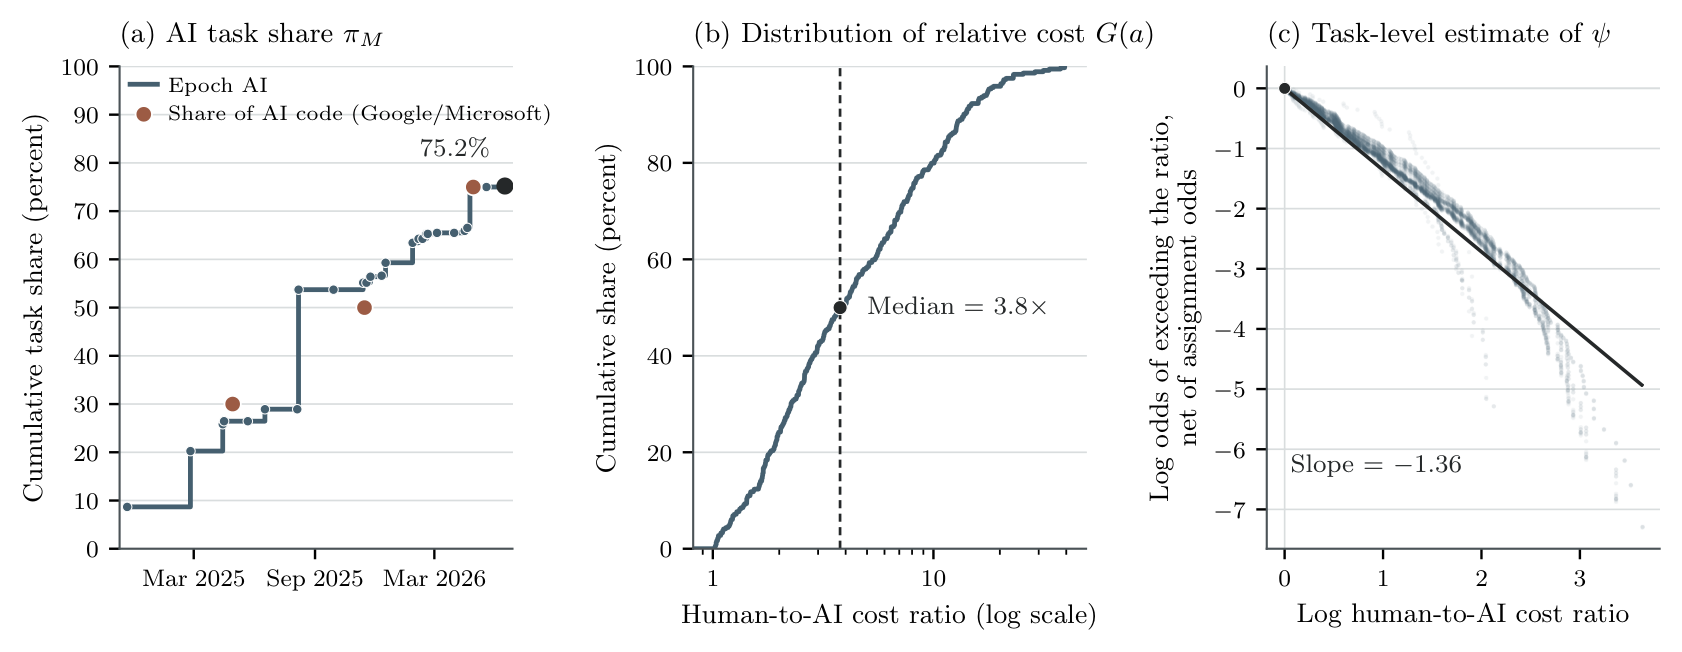
\includegraphics[width=1\textwidth]{empirics/exhibits/figure1_three_panels.png}

\vspace{0.25em}
 %
\begin{minipage}[c]{0.97\textwidth}%
{\footnotesize\textit{Notes:}}{\footnotesize{} Panel~(a) reports, by
release date, the share of the 484 tasks completed at a cost
below human cost. The final share is 75.2
percent. Three larger circle points show the shares of software written
by AI that two large software producers reported, the three values
to which the factor that stands for deployment costs beyond tokens
is calibrated. Panel~(b) plots the empirical distribution of the
human-to-AI cost ratio among tasks assigned to AI. Its horizontal
axis is on a log scale; the line and the point show that median human
cost is 4 times AI cost. Panel~(c)
plots the 6{,}589 points behind equation~\eqref{eq:task-regression},
one for each task and date, before winsorization: for each assigned
task, the log odds that the cost ratio of a task exceeds its observed
ratio, net of the log odds of assignment at that date, against the
log cost ratio. Each of the 26 release dates contributes
one line; the point at $d=1$ is cost parity, through which every
line passes by construction, and the fitted line with no intercept,
estimated after winsorization as in the text, has slope $-1.36$,
the task-level estimate of $-\psi$. Each panel uses the BLS wage
scaled up by 1.4, an upper limit of 16
hours, and the midpoint in logs of each range of hours. Panel~(a)
and panel~(c) follow the frontier by release date; panel~(b) uses
its June~2026 endpoint. Panel~(a) and panel~(b) show
no fitted distribution. Our calculation uses the task-level cost and
assignment data described in Appendix~\href{https://ahmadlp.github.io/Lashkaripour_AI_Displacement_Online_Appendix.pdf\#page=101}{D.1}.}%
\end{minipage}
\end{figure}


\paragraph{The relative cost distribution $G(.)$ is continuous.}

Even though we fit a Fréchet distribution to the data, the headline
result of the paper does not require Fréchet. AI-driven displacement
coincides with real wage growth so long as the human-to-AI cost distribution
$G(.)$ is continuous, as Theorem \ref{prop:general-displacement}
demonstrated. Figure \ref{fig:cost-spread-distribution} plots the
raw distribution $G(.)$ over tasks from the latest release date.
The plot visibly satisfies the continuity requirement posited by Theorem
\ref{prop:general-displacement}. Moreover, the Fréchet fit implied
by each estimate of $\psi$ closely mimics the empirical distribution,
suggesting that our quantitative framework also provides a reasonable
approximation of the data.

\begin{figure}[t]
\centering \caption{ Distribution of the Human-to-AI Cost Ratio across Tasks and the
Fréchet Fit}\label{fig:cost-spread-distribution}
\vspace{0.25em}
 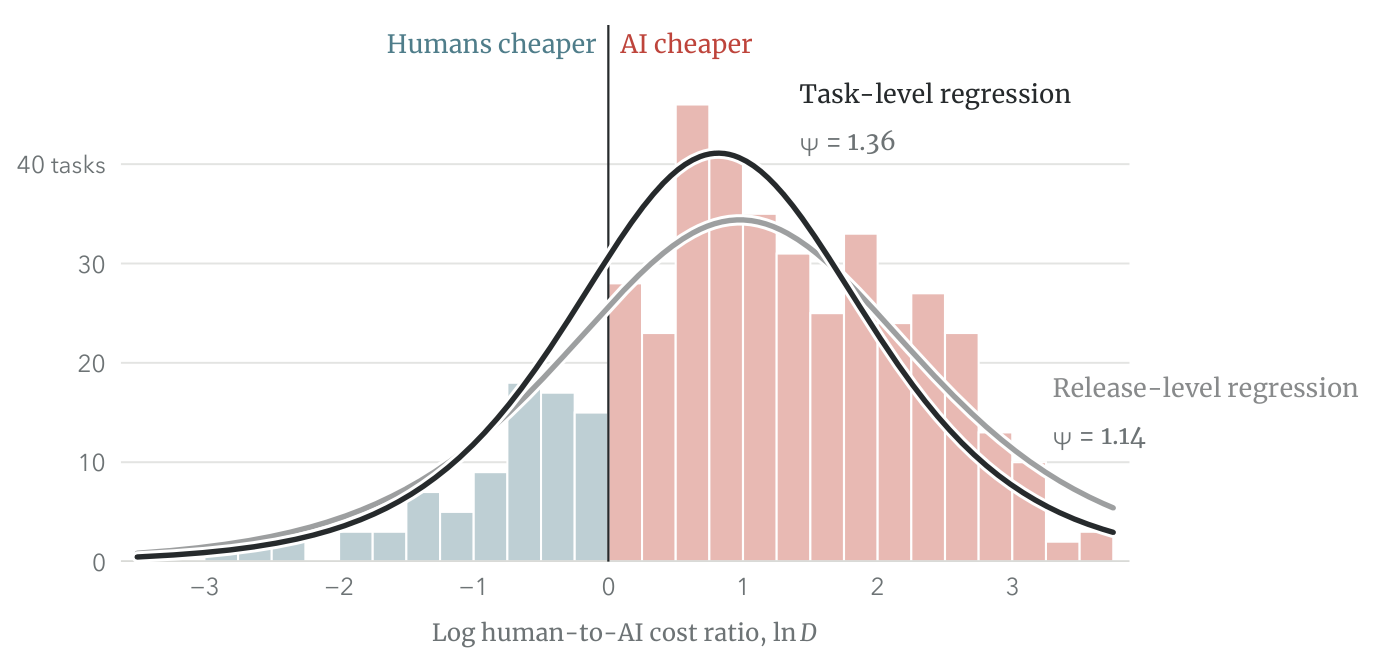
\includegraphics[width=0.98\textwidth]{empirics/exhibits/figure2_cost_spread_distribution.png}

\vspace{0.25em}
 %
\begin{minipage}[c]{0.97\textwidth}%
{\footnotesize\textit{Notes:}}{\footnotesize{} The figure shows the
distribution of the log human-to-AI cost ratio across the 484
tasks at the June~2026 endpoint of the AI frontier.
The AI cost frontier is determined by the cheapest successful completion
of each task. We treat uncompleted tasks as below cost parity but
do not draw them. The line at $D=1$ shows cost parity; the share
of tasks to its right is 75.2 percent.
Each fitted line is the density of the log cost ratio implied by the
paper's Fréchet distribution based on estimates of $\psi$ from Table
\ref{tab:two-estimates}: $1.36$ (task-level regression)
or $1.14$ (release-level regression). Its calibrated
so that its share above parity equals the observed share and scaled
to the number of tasks. Costs use the BLS wage scaled up by 1.4,
an upper limit of 16 hours, and the midpoint in logs
of each range of hours.}%
\end{minipage}
\end{figure}


\subsection{Discussion}

The parameter also governs the wage response to task displacement
and the gross reassignment hidden behind net displacement. First,
the model's real-wage equation implies
\begin{equation}
\frac{\partial\ln w_{t}}{\partial\ln(1/\pi_{L,t})}=\frac{1}{\psi}.\label{eq:measured-wage-selection-elasticity}
\end{equation}
At the two estimates of $\psi$, the local percentage increase in
the real wage is 0.7 to 0.9 times
the percentage contraction in labor's task share. This is an elasticity
with respect to labor's task share, not the response to a unit change
in AI's task share, which also depends on the level of assignment.

For the counterfactuals, we use the task-level distribution estimate
$\psi=1.36$ from Table \ref{tab:two-estimates} and impose this
value in every sector. Appendix \href{https://ahmadlp.github.io/Lashkaripour_AI_Displacement_Online_Appendix.pdf\#page=101}{D} discusses the
limits of applying the software-engineering estimate to other industries,
and Appendix Figure \href{https://ahmadlp.github.io/Lashkaripour_AI_Displacement_Online_Appendix.pdf\#page=105}{B1} reports estimates
under different wage bases and assessed-time conventions. Incomplete
tasks provide no AI cost observation, as Appendix \href{https://ahmadlp.github.io/Lashkaripour_AI_Displacement_Online_Appendix.pdf\#page=106}{D.5}
explains. These estimates describe observed comparative advantage
and do not determine its ultimate range.

\subsection{Macroeconomic Calibration}

We use the full model with multiple sectors, multiple factors, and
input-output linkages to run the simulations. As detailed in Appendix
\href{https://ahmadlp.github.io/Lashkaripour_AI_Displacement_Online_Appendix.pdf\#page=74}{C}, counterfactual equilibria can be simulated
by calibrating the model to six sufficient statistics from the baseline
equilibrium. Two of these statistics are industry-level share variables:
(1) Final consumption shares, $\beta_{s}$, and input-output shares,
$\Gamma_{ks}$, and (2) the share of tasks $\pi_{Ms}$ performed by
AI in that industry. The two other statistics correspond to worker
allocation under the status quo. Namely, (3) the share of each education
group employed in each industry, $\mu_{gs}$, and (4) each group's
share of the aggregate wage bill, $\omega_{g}$. The final requirements
two are structural parameters: (5) the productivity dispersion parameter,
$\psi$, and (6) the Roy parameter $\kappa_{g}$, which regulates
worker mobility across sectors.\footnote{To allow for capital income, the calibrated model lets final output
combine the task bundle $Y_{s}$ with fixed sector-specific capital
$K_{s}$. Namely, $\tilde{Y}_{s}=Y^{\theta_{s}}_{s}K^{1-\theta_{s}}_{s}$,
where $\theta_{s}>0$ is an observable share.} The counterfactual equilibrium can be solved using these observable
or estimable statistics by solving the system \href{https://ahmadlp.github.io/Lashkaripour_AI_Displacement_Online_Appendix.pdf\#page=88}{(C20)}--\href{https://ahmadlp.github.io/Lashkaripour_AI_Displacement_Online_Appendix.pdf\#page=89}{(C29)}
in changes.

The consumption and input-output shares, $\beta_{s}$, $\Gamma_{ks}$,
are calibrated to match the 2024 BEA accounts on input-output and
value added shares \citep{bea2026io}. the sample covers $71$
industries, with details about data construction provided in Appendix
\href{https://ahmadlp.github.io/Lashkaripour_AI_Displacement_Online_Appendix.pdf\#page=75}{C.2}. We calibrate the employment shares
$\mu_{gs}$ to the 2024 American Community Survey \citep{census2024pums}.
The sample includes employed adults aged 25--64 in private and government
sectors, with the latter accounting for $16.9$
percent of the wage bill. We group workers into (1) high school or
less, (2) some college or an associate degree, and (3) a bachelor's
degree or more. Their share $\omega_{g}$, of the aggregate wage bill
claimed by each group are respectively, $18.2$,
$21.4$, and $60.4$
percent. We adjust the group-by-industry wage bills to match the model's
sector wage bills while matching these group-level shares. We use
$\psi=1.36$ and, following \citet{gry2023}, set $\kappa_{g}=1.5$
for every group. Appendix \href{https://ahmadlp.github.io/Lashkaripour_AI_Displacement_Online_Appendix.pdf\#page=74}{C} reports further
details on the industry concordances and calibration method.\footnote{To allow for capital income, we calibrate the share of primary non
capital inputs as $\theta_{s}=\min\left\{ \frac{w^{D}_{s}L^{D}_{s}}{\pi_{Ls}\alpha_{s}X_{s}},1\right\} $,
where $w^{D}_{s}L^{D}_{s}$ is worker compensation in the data. In
our production function with capital, labor receives $\theta_{s}\alpha_{s}\pi_{Ls}X_{s}$,
agentic AI receives $\theta_{s}\alpha_{s}\pi_{Ms}X_{s}$, and sector-specific
capital receives $(1-\theta_{s})\alpha_{s}X_{s}$, where $X_{s}$
is gross revenue. The share $\theta_{s}$ is set to one in 8 sectors,
which leaves the aggregate model-predicted wage bill 1.29 percent
below the BEA reported worker compensation. We retain this accounting.
See Appendix \href{https://ahmadlp.github.io/Lashkaripour_AI_Displacement_Online_Appendix.pdf\#page=76}{C.3} for more details.}

The share $\pi_{Ms}$ of tasks performed by AI in each industry is
calibrated using the July 2026 survey of $1{,}103$
employed US adults by Epoch AI and Ipsos \citep{epochpolling2026}.
We supplement this data the Anthropic Economic Index \citep{massenkoffmccrory2026labor}
to extend that measurement beyond the survey. The Epoch AI--Ipsos
survey asks US workers how much they rely on AI for 10 types of tasks,
such as reading documents and analyzing data. These tasks, however,
represent only a fraction of the work people perform. So, we rely
on the Anthropic Economic Index to extend coverage to further tasks.
Anthropic covers a wider range of tasks scoring them based on Claude
and assessed AI capability. The drawback is that these scores do not
directly measure the percentage of work delegated to AI. Yet they
can be used to impute the AI task share $\pi_{Ms}$ across work that
is not represented in the Epoch AI--Ipsos survey.

We build each $\pi_{Ms}$ from industry worker occupation mix in industry
$s$ as follows. The Epoch AI--Ipsos survey measures AI use across
ten tasks, identifying each respondent’s occupation group. Each occupation
performs many tasks not included in the survey. So, we draw on O{*}NET’s
task descriptions to map tasks to occupation \citep{onet2026}. We
then impute AI use on the remaining tasks per acceptation. For this,
we leverage the fact that in the Anthropic Economic Index, the average
score for tasks outside the Epoch AI--Ipsos survey is $0.66$
times the surveyed tasks. We impose a proportionality assumption,
whereby AI performs the non-surveyed tasks in each occupation at $0.66$
times that occupation’s surveyed rate.

Figure \ref{fig:sector-landscape} provides an overview of the $71$
industries. Each circle represents one industry, with the size scaled
with the industry’s value added share, and the colors running from
orange to teal based on the share of employees with college degrees
or higher. Panel A displays the intensity by which production in industry
uses cognitive versus physical tasks. Industries located in the bottom
right of the plot rely more on cognitive skills, while industries
located in top left involve more physical work.\footnote{The manual and cognitive task indexes are not input shares in production
function aggregating over tasks. They are different indexes and do
not add up to 100.} Panel B compares two measures of AI exposure. It plots the current
AI task share $\pi_{Ms}$ against the forward-looking exposure score
$e_{s}$ on the horizontal axis. The latter is constructed from \citep{emmr2024}
based on the assessment of whether large language models could reduce
task completion time by one-half without reducing quality.\footnote{A task receives an exposure score of 1 if a large language model by
itself could deliver the time cost reduction. It receives a score
of 0.5 if the time cost reduction requires additional software built
around the model, and 0 otherwise. They map these task-level ratings
into exposure scores for each occupation. We map these occupation
scores to industry-level scores using employment shares.} The two exposure measures serve different purposes: the survey-based
$\ensuremath{\pi_{Ms}}$ determines the baseline AI task share in
the calibrated model, while $e_{s}$ is an ex-ante measure that proxies
for the adoption rate, which is the share of future AI improvements
a sector can absorb.\footnote{Weighted by value added, the average AI adoption to date is $14.2$
percent and the average exposure is $35.2$
percent, with $\pi_{Ms}<e_{s}$ in every industry. The survey covers
$10.25$ percent of tasks directly, weighted
by employment, and drawing occupations at random gives an aggregate
share between $11.8$ and $17.3$
percent. Appendix \href{https://ahmadlp.github.io/Lashkaripour_AI_Displacement_Online_Appendix.pdf\#page=93}{C.11} runs the counterfactuals
with Microsoft's lower share of $6.8$
percent, where the five year real wage gain falls to $6.7$
percent under balanced adoption and $7.7$
percent under jagged adoption.} Appendix \href{https://ahmadlp.github.io/Lashkaripour_AI_Displacement_Online_Appendix.pdf\#page=74}{C} details the construction of these
measures, and Appendix \href{https://ahmadlp.github.io/Lashkaripour_AI_Displacement_Online_Appendix.pdf\#page=93}{C.11} runs sensitivity
analyses using the lower baseline exposure shares based on Microsoft's
record of AI use.

\begin{figure}[t]
\centering \caption{Sectoral heterogeneity in cognitive skill intensity and AI exposure}
\label{fig:sector-landscape} \vspace{0.25em}
 % inside_import 
% before   
% ignored 
% args [width=0.98\textwidth]
% full_filename quantification/exhibits/sector_profiles/figure_sector_landscape.pdf
% after 
 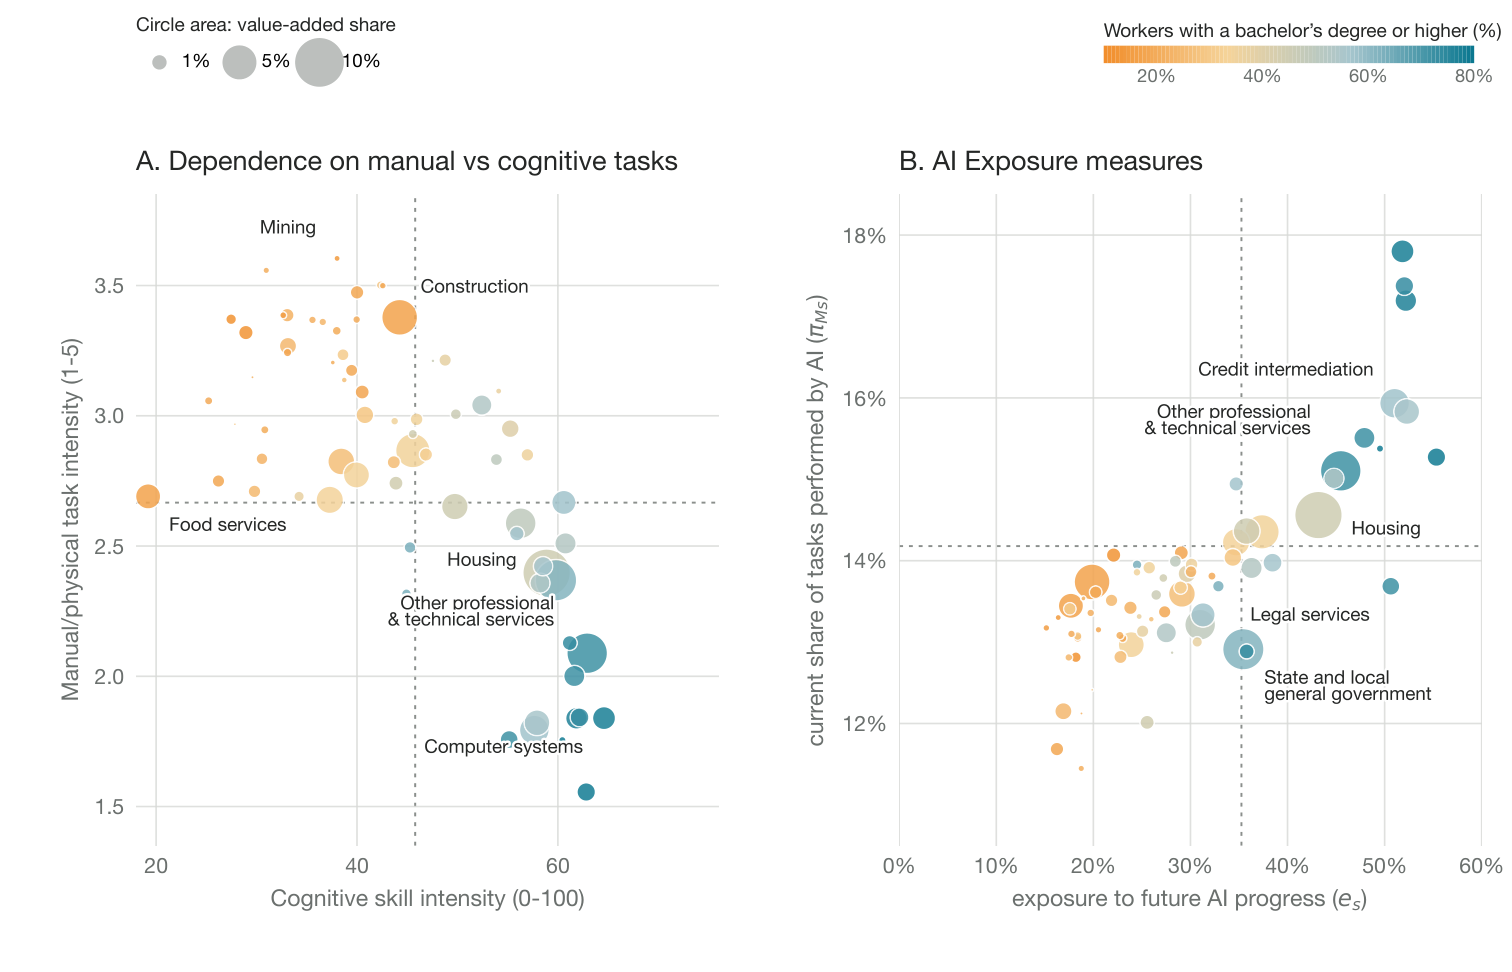
\includegraphics[width=0.98\textwidth]{quantification/exhibits/sector_profiles/figure_sector_landscape.png}

\vspace{0.25em}
 %
\begin{minipage}[c]{0.94\textwidth}%
{\footnotesize\textit{Notes:}}{\footnotesize{}
Each circle represents one sector. Panel A plots the physical intensity
index against the cognitive skill intensity index on the horizontal
axis. The dashed lines report the employment weighted mean for each
axis. Panel B plots the current AI task share against the exposure
measure used to discipline adoption of growing AI capabilities. The
dashed lines represent the value added weighted mean for each axis.
In each panel, circle size shows the sector's value added share, and
the colors report the share of its workers with a bachelor's degree
or more. The calculations are based on the 2024 BEA input--output accounts,
the Epoch AI--Ipsos survey, Anthropic Economic Index task data, May
2025 BLS employment, the 2025 BLS employment projection and skill
scores, O{*}NET 31.0, the 2024 American Community Survey, and occupation
exposure ratings \citep{bea2026io,epochpolling2026,bls2026oews,bls2026ep,onet2026,census2024pums,emmr2024}.}%
\end{minipage}
\end{figure}


\subsection{ Historical Validation: The Model Explains 2022-25 Labor Market
Effects}\label{sec:model-validation}

Before deploying the estimated model for forward-looking counterfactual
simulations, it is useful to test its explanatory power with respect
to observed AI displacement effects. To this end, we perform a retrospective
test of the model using IV-based goodness-of-fit measure developed
by \citet{adao2025test}. We ask whether the calibrated model reproduces
the labor market effects that materialized between 2022 and 2025,
but were not targeted in the calibration. As detailed in Appendix
\href{https://ahmadlp.github.io/Lashkaripour_AI_Displacement_Online_Appendix.pdf\#page=93}{C.12}, we use changes to sectoral wages from
May 2022 to May 2025 as our validation test target.

The test has a simple logic. Between 2022 and 2025, the economy was
hit by many shocks, each of which may have affected wages. One such
shock was the rapid improvement in agentic AI capabilities from near-zero
levels to those observed in 2025. This rapid growth shock hit different
sectors with various levels of intensity, represented by instrument
$z_{s}$. The idea behind the test is to use the calibrated model
to simulate the wage changes $\{\Delta w_{s}\}$ implied by AI growth.
We then define the residual wage change as the difference between
observed wage growth from 2022 to 2025 and the model-predicted wage
change due to AI, $\Delta w^{D}_{s}-\Delta w_{s}$. If the model correctly
predicts the wage effects of AI growth, this residual should be orthogonal
to the AI growth shock. Formally, the goodness of fit statistic $\widehat{\beta}_{z}=S^{-1}\sum_{s}z_{s}(\Delta w^{D}_{s}-\Delta w_{s})$
must have an expected value of zero. If so, the residual reflects
other contemporaneous shocks hitting the economy, rather than omitted
wage effects of AI growth the model failed to capture. The corresponding
IV coefficient is
\[
\widehat{\beta}^{IV}=\frac{S^{-1}\sum_{s}z_{s}\Delta w^{D}_{s}}{S^{-1}\sum_{s}z_{s}\Delta w_{s}}=1+\frac{\widehat{\beta}_{z}}{S^{-1}\sum_{s}z_{s}\Delta w_{s}},
\]
From the lens of the model, the change in the AI task share $\Delta\pi_{Ms}$
in each sector $s$ is the sufficient statistics for constructing
the instrument $z_{s}$ and simulating $\Delta x_{s}$. The change
in task share is constructed based on each sector's May 2022 occupation
mix with the measure of occupational exposure to agentic AI from \citet{emmr2024}.
Appendix \href{https://ahmadlp.github.io/Lashkaripour_AI_Displacement_Online_Appendix.pdf\#page=93}{C.12} provides the details about the
data construction and inference.

Because we are analyzing a three years window, labor mobility is presumably
less than implied by $\kappa=1.5$, which estimated based on
labor market response over a longer horizon. We therefore assess two
cases: $\kappa\downarrow1$, in which workers are frozen in their
original sectors, and $\kappa=1.5$, following the preferred
estimation value of \citet{gry2023}. Figure \ref{fig:model-validation}
reports the wage effects and the IV slope test. The goodness-of-fit
statistic is $\widehat{\beta}_{z}=1.7\times 10^{-4}$
under $\kappa\downarrow1$ and $\widehat{\beta}_{z}=-8.6\times 10^{-5}$
with $\kappa=1.5$. The null of a zero discrepancy is not rejected
at the 5 percent confidence level, in both cases. The corresponding
IV coefficient is $\widehat{\beta}^{IV}=0.8$
when workers remain in their original sectors, with a 95 percent confidence
set of $[0.43,1.21]$.
With $\kappa=1.5$, the IV coefficient is $\widehat{\beta}^{IV}=1.15$,
with a 95 percent confidence set of $[0.62,1.74]$.
Both confidence sets contain one.

\begin{figure}[!tbh]
\centering \caption{Observed 2022-25 Wage Changes Are Consistent with the Model Predictions}
\label{fig:model-validation} \vspace{0.25em}
 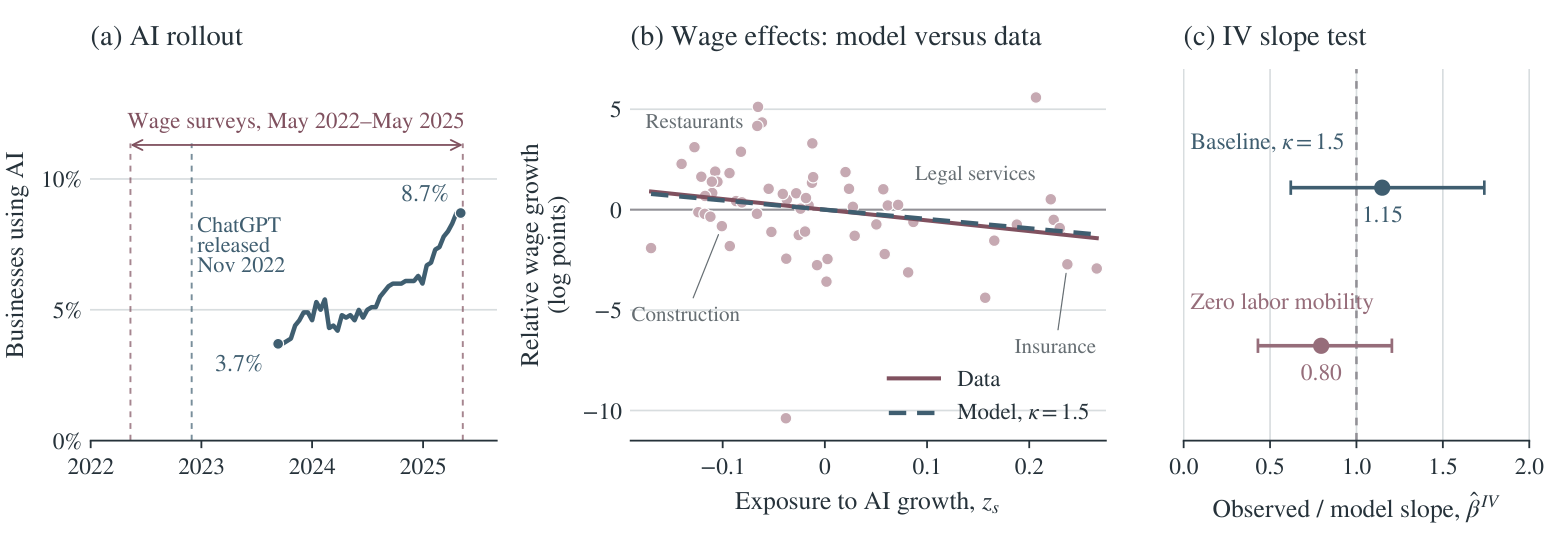
\includegraphics[width=0.98\textwidth]{quantification/validation_acd/exhibits/figure_model_validation.png}

\vspace{0.25em}
 %
\begin{minipage}[c]{0.94\textwidth}%
{\footnotesize\textit{Notes:}}{\footnotesize{}
Panel (a) plots Census business AI use. The model task share is scaled
from $14.2$ percent in July 2026 to $5.7$
percent in May 2025. The scaling ratio, $0.087/0.217$,
is approximate because the survey wording changed. The model compares
the May 2025 equilibrium with near-zero AI use, which is assumed for
May 2022. Panel (b) shows $61$ sectors.
Nominal wage changes use fixed May 2022 occupation weights. Wage changes
and exposure are demeaned across these sectors. The lines project
observed and model-predicted wage changes on the same exposure instrument;
the comparison concerns relative wage effects. In panel (c), the dashed
line marks equal slopes, and the intervals are 95 percent Anderson--Rubin
confidence sets. The comparison does not test the average wage change,
employment, or welfare, and the confidence sets are wide enough to
allow sizable errors in the predicted changes. Appendix \href{https://ahmadlp.github.io/Lashkaripour_AI_Displacement_Online_Appendix.pdf\#page=93}{C.12}
describes the construction and the checks on the inference.}%
\end{minipage}
\end{figure}


\section{Forward-Looking Impacts of AI-Driven Growth}\label{sec:counterfactuals}

This section uses the calibrated model to simulate the prospective
impacts of AI-driven growth, assuming AI progress continues along
its current trajectory. Our goal is to isolate the pure impact of
AI-driven growth on the labor market through Ricardian comparative
advantage. We therefore shut down all other engines of growth, including
population growth and capital investment. This naturally comes with
clear caveats: fertility rates and investment decisions are presumably
influenced by AI-driven growth, which is not modeled here. Ricardian
reassignment is also not the only force affecting labor market outcomes,
though the retrospective test of the model's predictive power points
to its ability to isolate AI-driven growth effects, at least over
a shorter time horizon. We begin by describing how we model the prospective
AI growth trajectory, then present four results tightly connected
to our theoretical framework.

\subsection{Extrapolating the AI Growth Trajectory}

We extrapolate the trajectory of future AI growth from the observed
decline in the cost of completing software engineering tasks. The
data used to estimate the rate of cost decline is the same as Section
\ref{sec:measurement}. To give context, the data record the cost
of AI systems performing software tasks. The cost per successful task
is calculated based on fixed token prices from July 31, 2026. The
reduction in cost therefore represent pure improvement in token efficiency.
This is of course a conservative measurement stance, since technological
progress can present itself in terms of lower token costs. However,
we focus our measurement on fixed token prices to disentangle pure
technological progress from competition and captive pricing strategies.

Figure \ref{fig:ai-cost-path} plots the resulting cost index over
the running sample period. Task costs at fixed token prices fell at
an annual rate of $79.1$ percent 19 months of
model releases. We assume that AI task costs continue to fall, but
that the annual rate of decline slows from $79.1$
percent initially to about $45.8$
percent after five years. This calculation follows from improvements
in computer hardware halving the cost of completing tasks every 1.7
years. Meanwhile the cost reducing effects of improvements in model
training, model design, and harness halve every two years.\footnote{Specifically, we model the rate of decline in the task cost $g(t)\equiv-d\ln c(t)/dt$
as $g(t)=g_{H}+(g_{0}-g_{H})2^{-t/2},$ where $g_{0}\approx1.57$
is the estimated current growth rate and $g_{H}=\ln(2)/1.7$ is the
rate implied by hardware improvements.} Under these assumptions, task costs fall by $99.2$
percent after five years.\footnote{With the rate of decline held at its current level, the cost of performing
tasks with agentic AI tools would fall by $99.96$
percent.} Appendix \href{https://ahmadlp.github.io/Lashkaripour_AI_Displacement_Online_Appendix.pdf\#page=85}{C.4} unpacks more details about
the our extrapolation of the growth trajectory.

\begin{figure}[!tbh]
\centering \caption{The Cost of Completing the Same AI Task Fell by About 79 Percent per
Year}
\label{fig:ai-cost-path} \vspace{0.25em}
 % inside_import 
% before   
% ignored 
% args [width=0.98\textwidth]
% full_filename quantification/exhibits/figure_ai_cost_path.pdf
% after 
 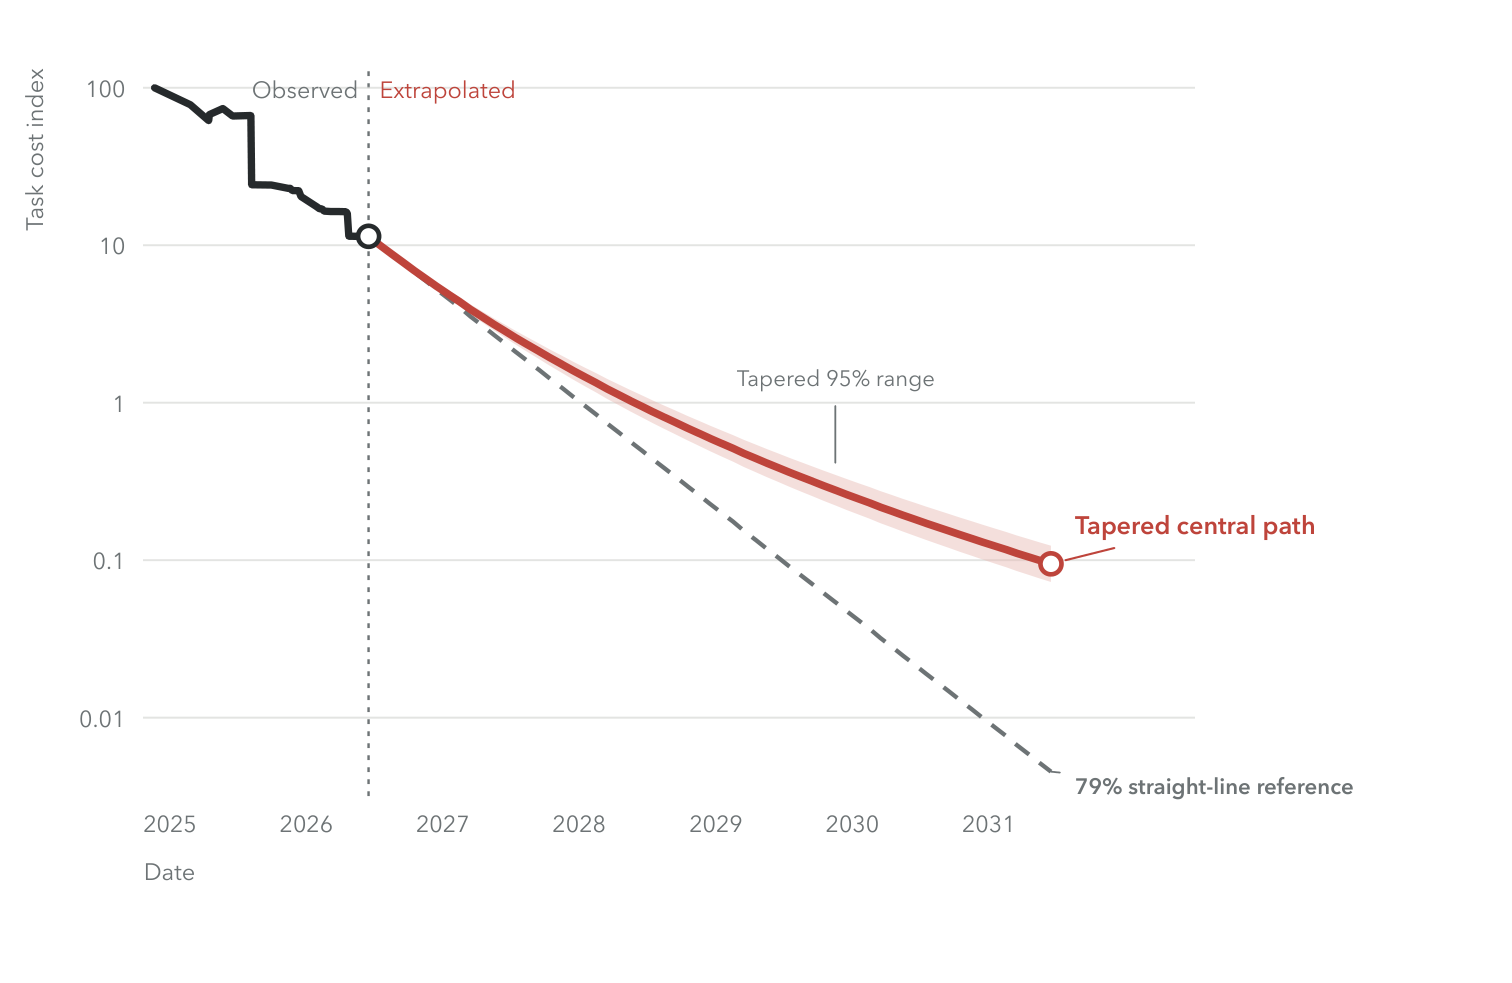
\includegraphics[width=0.98\textwidth]{quantification/exhibits/figure_ai_cost_path.png}

\vspace{0.25em}
 %
\begin{minipage}[c]{0.94\textwidth}%
{\footnotesize\textit{Notes:}}{\footnotesize{} The observed cost index
is calculated by release date from the frontier of the cheapest successful
completion of each task, with task fixed effects, and equals 100 at
the first release date. Every model uses the same fixed token prices.
The solid projection assumes that the annual rate of decline slows
toward the rate of improvements in computer hardware; the range above
and below it uses the same assumption for the 95 percent confidence
set. The line below the solid projection holds the estimated 79
percent annual decline constant. The cost index is on a log scale.
Section~\ref{sec:measurement} describes the task panel and the estimation.
Our calculation uses SWE-bench Verified model task costs~\citep{jimenez2024,openai2024verified}.}%
\end{minipage}
\end{figure}

Next, we infer the growth in the stock of frontier AI knowledge from
the reduction in average task cost performed by AI. For this, we invoke
the observation that under the model's Fréchet distribution, the average
task cost for AI is
\[
c_{M}=\int^{1}_{0}c_{M}(i)\,di=\Gamma\!\left(1+\frac{1}{\theta}\right)rT^{-1/\psi}_{M}
\]
 Hence, our measure of average task cost reduction at token prices
fixed in units of the final good ($\hat{r}=1$) determines the growth
in stock of AI knowledge as $\hat{T}_{M}=\widehat{c}^{-\psi}_{M}$.
We assume that sector $s$ experiences $e_{s}$ times the decline
in log AI costs, where $e_{s}$ is an exposure measure obtained from
interacting the occupation exposure ratings from \citep{emmr2024}
with BLS sectoral occupation employment weight. Thus, the sector's
average AI cost and technology therefore change by
\begin{equation}
\hat{T}_{Ms}=\hat{c}^{-\psi e_{s}}_{M}.\label{eq:counterfactual-shocks}
\end{equation}
We also experiment with a balanced adoption scenario, which replaces
$e_{s}$ with the weighted mean exposure $\bar{e}=\sum_{k}\alpha_{k}\lambda_{k}e_{k}$,
where $\alpha_{k}\lambda_{k}$ are value added shares.

\subsection{Real Wage Growth Despite AI-Driven Displacement}

Figure \ref{fig:aggregate-real-wage-labor-share} shows how average
real wages and labor's share of GDP change under our projected AI-driven
growth scenario. The picture shows a clear divergence, amplifying
the view expressed at the outset of this paper---that displacement
does not lead to immiserization. Our simulation predicts that after
five years, average real wages rise by $18.5$
percent, while labor's share of value added falls from $54.1$
to $39.9$ percent. On an
accounting level the explanation is straightforward. After five years,
real output rises by $60.7$
percent, while workers' share of value added falls from $54.1$
to $39.9$ percent. With the
number of workers held fixed, these changes still imply an $18.5$
percent increase in average real wages. To illustrate the key role
jaggedness in AI capabilities, the lighter lines in Figure \ref{fig:aggregate-real-wage-labor-share}
repeat the simulation with an AI frontier five times less jagged ($\psi\rightarrow5\psi$).
Real output rises by $102.8$ percent
after five years, more than the baseline with greater jaggedness,
yet average real wages barely change, and labor's share of value added
falls more aggressively to $26.9$
percent, about $50$ percent
of its value today.

\begin{figure}[!tbh]
\begin{centering}
\centering \caption{Average Real Wages Rise Despite the Sharp Drop in Labor's Share of
GDP}\label{fig:aggregate-real-wage-labor-share}
 \hspace*{-30pt}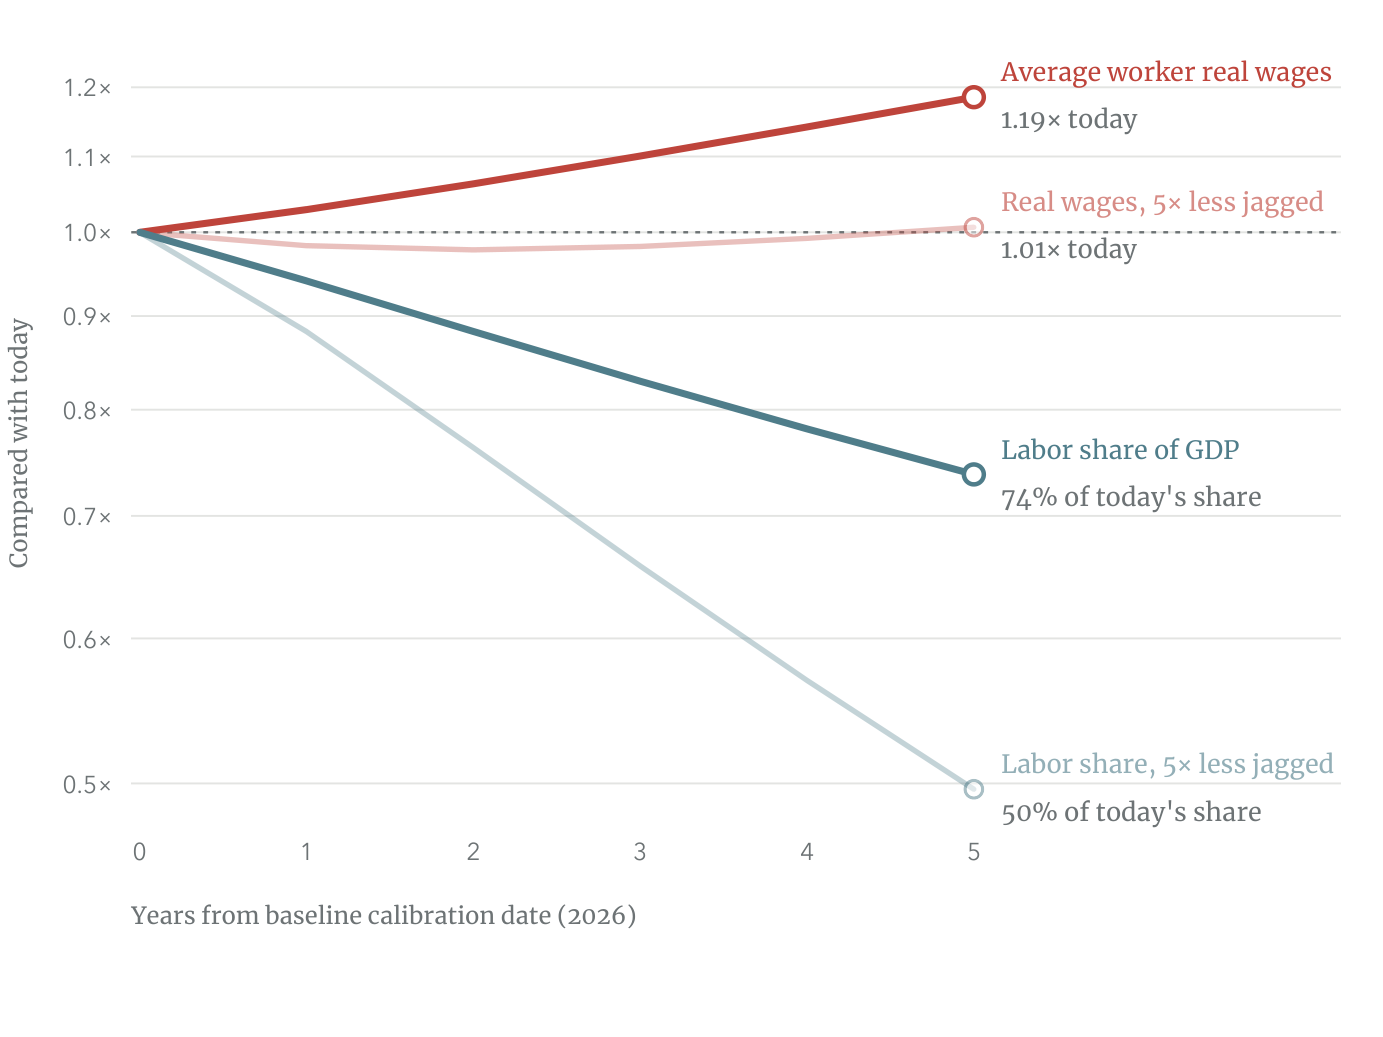
\includegraphics[width=1.1\textwidth]{quantification/exhibits/figure_aggregate_real_wage_labor_share.png}
\par\end{centering}
\vspace{0.25em}
 %
\begin{minipage}[c]{0.94\textwidth}%
{\footnotesize\textit{Notes:}}{\footnotesize{} Each line is relative
to its value today and equals one at year zero, on a log scale. The
darker lines use the estimated jaggedness of the AI frontier, $\psi=1.36$;
the lighter lines repeat the simulation with a frontier five times
less jagged, $\psi=6.79$, and everything else unchanged.
Aggregate real wages are the mean of the three education groups' real
wages, weighted by baseline wage bills. The teal line is workers'
share of total value added. The figure reports it as a percentage
of the share today. The numeraire is the model's final expenditure
bundle for the full set of industries. The simulation uses the central
cost path in Figure~\ref{fig:ai-cost-path}, holds the stock of AI
capacity fixed, and sets the change in each sector's AI technology
as in equation~\eqref{eq:counterfactual-shocks}. Our calculation
uses the Epoch AI--Ipsos survey, O{*}NET, the BEA industry accounts,
BLS employment, the 2024 American Community Survey, and occupation
exposure ratings~\citep{epochpolling2026,onet2026,bea2026io,bls2026oews,census2024pums,emmr2024}.}%
\end{minipage}
\end{figure}

The more interesting explanation is derived from the Ricardian assignment
model. As labor gets displaced from 30\% of the tasks two development
follow. First, AI-performed tasks become more productive and their
output becomes cheaper as a result. Labor sorts into more productive
tasks, and the marginal product of labor grows. The labor becomes
more productive on the margin, and the wage buys a larger basket of
goods. Altogether, the real earning power of the workers grows, even
though they perform fewer tasks.

\subsection{Jagged versus Balanced AI Adoption}

Our baseline simulation allows adoption to be jagged, in the sense
that different sectors have different adoption rates. We proxy for
adoption rates, based on exposure measures inferred from the mix of
occupations a sector employs. It's motivated by evidence that the
tasks performed by some occupations are more amenable to AI automation
than others. A question worth exploring, here, is how jagged adoption
is contributing the real wage growth. Theorem 4 argued that jagged
adoption is generally better for \emph{aggregate} real wages. The
intuition is that jagged adoption enables sizable efficiency gains
in exposed sectors, which translate to lower prices for their goods,
while also presenting labor with shelter in lagging sectors and occupations.

Figure \ref{fig:real-wage-growth} compares the growth in aggregate
real wage under balanced and jagged AI adoption over the 5-year horizon.
Both cases use the same average cost decline projection, $\hat{c}_{M}$.
However, the balanced adoption applied this cost reduction uniformly
to all industries or occupations: $\hat{T}_{Ms}=\hat{c}^{-\psi\bar{e}}_{M}$
where $\bar{e}=\sum_{k}\alpha_{k}\lambda_{k}e_{k}$ is the weighted
average exposure. The results are similar over the first five years:
under balanced adoption, average real wages rise by $16.8$
percent and labor's share of value added falls to $39.6$
percent. Real output rises by $59.5$
percent under balanced adoption and $60.7$
percent under jagged adoption, so jagged adoption pays workers more
at about the same output growth. After five years, the difference
in annual wage growth increases every year. By year $50$,
real wages grow by $5.7$ percent
a year under balanced adoption and $8.9$
percent under jagged adoption. Workers move toward sectors where AI
improves more slowly. The prices of goods produced in these sectors
rise relative to prices in sectors where AI improves faster, increasing
the purchasing power of workers' earnings, as in Theorem \ref{thm:breadth}.

\begin{figure}[!tbh]
\centering \caption{Jagged AI Adoption Lifts \emph{Average} Real Wages Faster But has
stronger Distributional Effects}
\label{fig:real-wage-growth} \vspace{0.25em}
 % inside_import 
% before   
% ignored 
% args [width=0.98\textwidth]
% full_filename quantification/exhibits/figure_real_wage_growth.pdf
% after 

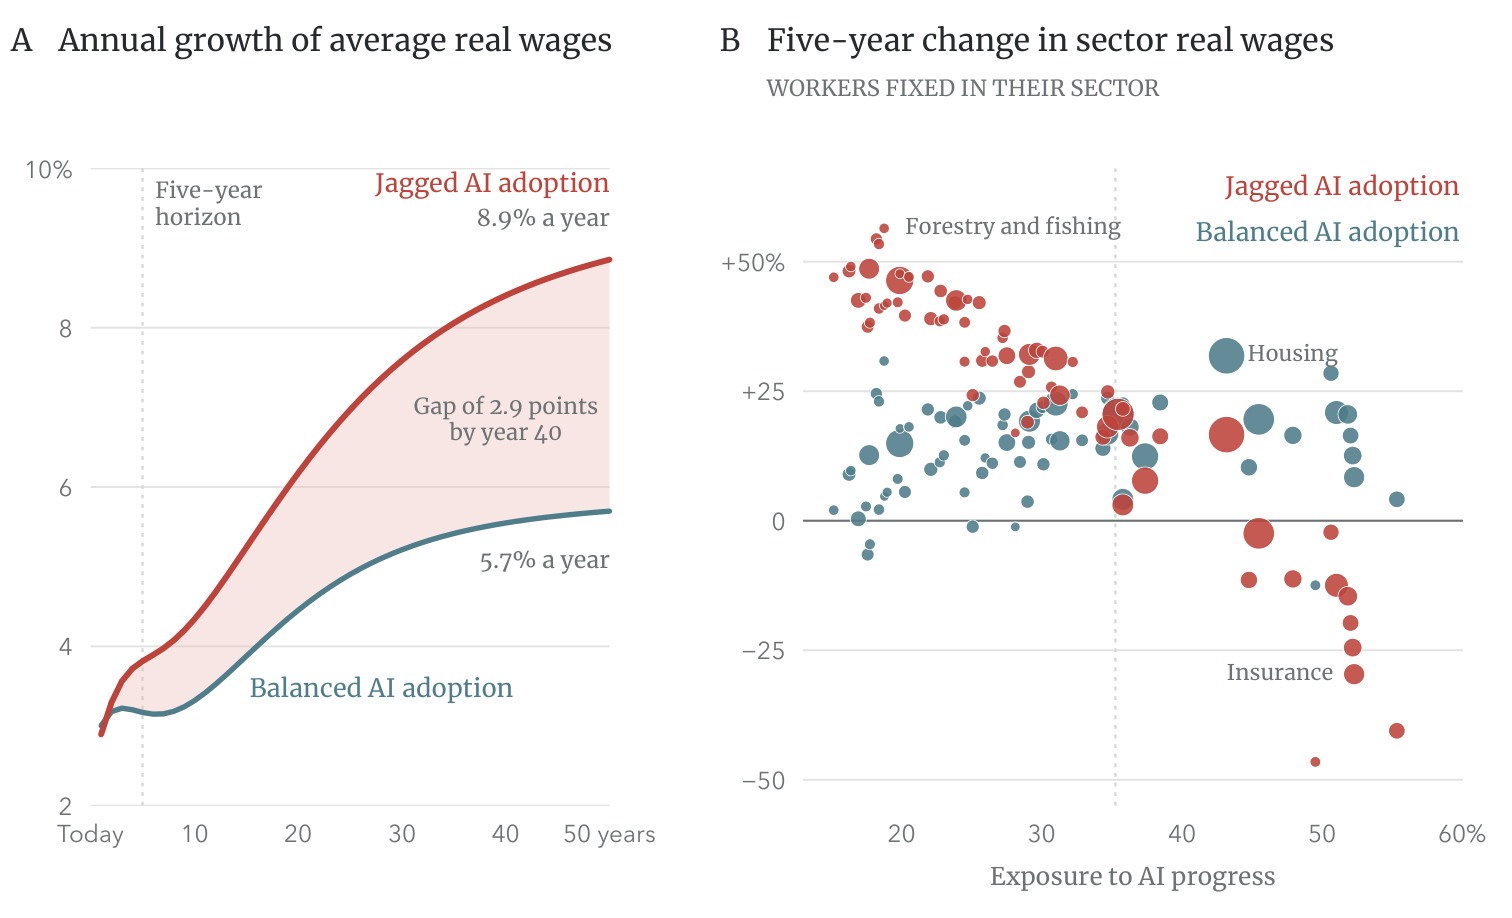
\includegraphics[width=0.98\textwidth]{quantification/exhibits/figure_real_wage_growth.png}

\vspace{0.25em}
 %
\begin{minipage}[c]{0.94\textwidth}%
{\footnotesize\textit{Notes:}}{\footnotesize{} In panel A, each line
is the annual growth rate of average real wages, the percentage change
from the previous year. Aggregate real wages are the mean of the three
education groups' real wages, weighted by baseline wage bills, in
units of the model's final expenditure bundle for the full set of
industries. The panel shows the gap between the two profiles, and
the rule shows the five-year horizon of the main results. Panel B,
plots a sector's change in real wages after five year against the
sector's exposure to AI progress when workers remain in their original
sectors. The area of each dot is proportional to the sector's value
added, and the dotted line marks the weighted average exposure across
sectors. Both the jagged and balanced scenarios use the cost reduction
path in Figure \ref{fig:ai-cost-path} for $50$
years, and set the change in each sector's AI technology as in equation
\eqref{eq:counterfactual-shocks}. Our calculation uses the Epoch
AI--Ipsos survey, O{*}NET, the BEA industry accounts, BLS employment,
the 2024 American Community Survey, and occupation exposure ratings~\citep{epochpolling2026,onet2026,bea2026io,bls2026oews,census2024pums,emmr2024}.}%
\end{minipage}
\end{figure}


\subsection{All Skill Groups Gain Irrespective of Mobility}

A notable result from our Ricardian theory is that all workers can
gain from AI-driven growth, irrespective of which sector they work
in, even if they cannot switch sectors. The prerequisite for this
to happen is that AI adoption not be too jagged and the agentic AI
and labor profiles be sufficiently different across tasks. Here we
test this using the full-fledged quantitative model with three groups
of workers based on educational levels: (1) high school or less, (2)
some college, and (3) Bachelor's degree or higher. We simulate the
average real wage for each group under our 5-year AI-driven growth
scenario.

Panel A in Figure \ref{fig:sector-mobility-floor} shows that average
real earnings rise among each education group even when workers cannot
move sectors. Panel A compares the five-year real wage gains in two
scenarios: in the first scenario workers remain in their original
sectors, which corresponds to $\kappa\downarrow1$. In the second
scenario, workers move across sectors, governed by the Roy parameter
$\kappa=1.5$. Without sectoral mobility, real earnings rise by $31.2$
percent among workers with high school degrees or less, $24.1$
percent for those with some college or an associate degree, and $12.5$
percent for those with a bachelor's degree or higher. When workers
can move between sectors, the corresponding real wage gains are $28.1$
percent, $22.9$ percent, and $14.1$
percent, respectively.\footnote{Appendix Figure \href{https://ahmadlp.github.io/Lashkaripour_AI_Displacement_Online_Appendix.pdf\#page=91}{C5} reports
the group-level gains when AI adoption is set to be balanced across
sectors.}

\begin{figure}[!tbh]
\centering \caption{All Education Groups Gain from AI-Driven Growth by Switching Tasks
rather than Sectors}
\label{fig:sector-mobility-floor} 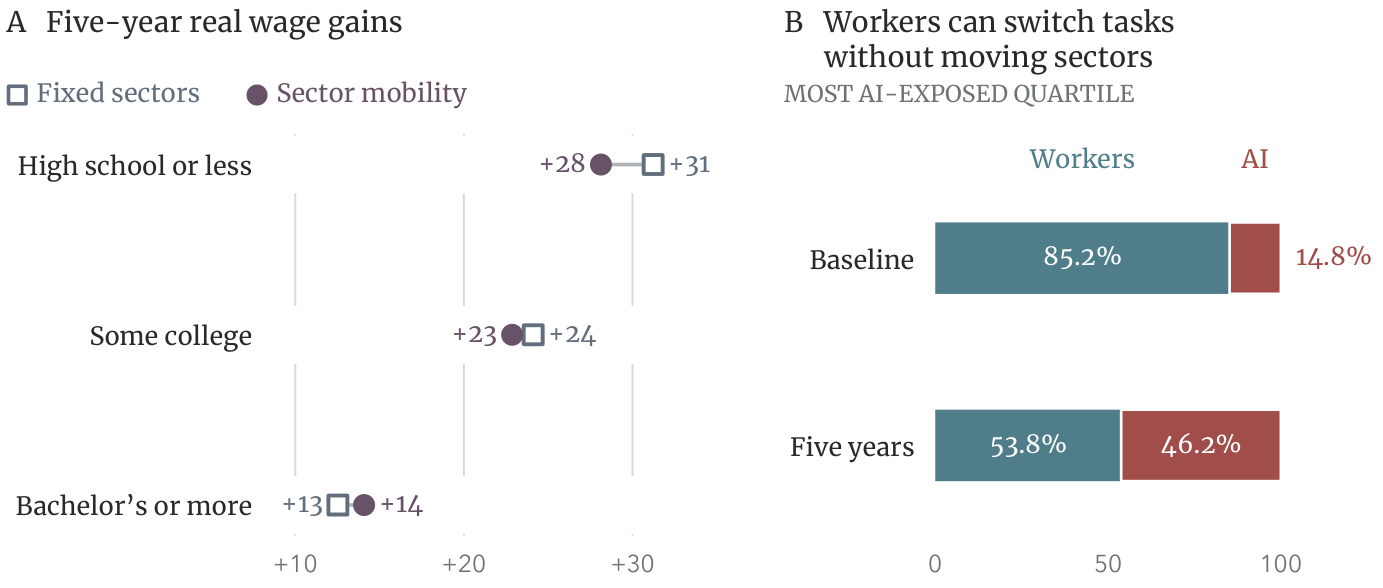
\includegraphics[width=0.98\textwidth]{quantification/exhibits/figure_education_earnings_gap.png}
\vspace{0.25em}
 %
\begin{minipage}[c]{0.94\textwidth}%
{\footnotesize\textit{Notes:}}{\footnotesize{} Panel A reports five-year
gains in the average real income of each education group. Open points
show the equilibrium in which workers remain in their original sectors,
and solid points show the equilibrium in which workers move across
sectors, at the calibrated $\kappa=1.5$. Panel B reports worker
and AI task shares, weighted by baseline value added, at baseline
and after five years for the $18$ sectors
with the highest AI exposure. The weights are scaled to sum to one
within this group. When workers remain in their original sectors,
the effective labor each education group supplies to each sector remains
at its baseline level. Sector assignments are therefore fixed, but
tasks may still shift between labor and AI within a sector; wages,
task shares, and sector prices adjust in general equilibrium. Each
panel holds the stock of AI capacity fixed. Our calculation uses the
Epoch AI--Ipsos survey, O{*}NET, the BEA industry accounts, BLS employment,
the 2024 American Community Survey, and occupation exposure ratings~\citep{epochpolling2026,onet2026,bea2026io,bls2026oews,census2024pums,emmr2024}.}%
\end{minipage}
\end{figure}

The reason workers gain despite not being able to switch sectors reflects
how AI displacement works. Unlike trade-driven displacement, AI-driven
displacement generally does not consume the entire task spectrum within
a sector. Instead, it leaves some niche tasks to workers. So, rather
than having to switch sectors to find work, workers simply sort into
those niche tasks within the same sector. Panel B in Figure \ref{fig:sector-mobility-floor}
illustrates this point. Among the $18$ sectors
with the highest AI exposure, workers' share of tasks falls from $85.2$
to $53.8$ percent over the five
year window, with AI's share rising from $14.8$
to $46.2$ percent. These results reveal
that, unlike say past trade shocks, AI-driven growth would mostly
affect labor market outcomes through within-sector rather than across-sector
reassignment. Even the most AI-exposed sectors continue to offer a
considerable range of tasks in which humans retains a comparative
advantage.

\subsection{The Illusive Jevons Paradox}

Next, we use the model to uncover the conditions under which the Jevons
paradox would emerge. Our baseline calibration assigns a unit elasticity
of substitution across sectors. As noted in Section \ref{sec:jevons}
, this expectedly leads knowledge workers, who hold BA degrees or
higher, to experience relatively smaller gains from AI-driven growth.
The reason is that the elasticity of substitution between knowledge
workers and AI is larger than the elasticity of substitution across
sectors. Consequently, the efficiency gains in knowledge-intensive
sectors do not generate a strong enough demand boost for those sectors
to offset the wage losses from AI substitution. However, if the inter-sectoral
elasticity of substitution is large enough, the demand boost could
be enough to more than offset the negative wage effects of AI displacement.

Figure \ref{fig:jevons-threshold} illustrates this point. It reports
the real wage gains over the five-year window for each education group
under different inter-sectoral substation elasticities, $\eta$. Under
the baseline calibration, $\eta=1$, the gains have the expected ordering,
workers with high school education or less gains the most, and those
with a bachelor's degree or higher gains the least for AI-driven growth.
The gap closes as $\eta$ rises and all groups experience the exact
same real wage gains under $\eta\approx2.5$, standing
at $28.9$ percent.\footnote{The elasticity at which the gap closes is a little above the threshold
$1+\psi\approx2.36$ noted in Section \ref{sec:jevons}
because the calibrated model is more general; it accounts for input-output
linkages and sector-specific capital.} Above this threshold we begin witnessing the Jevons paradox. Real
wages go up the most for workers with Bachelor's degrees or higher
who are the most exposed to AI-driven displacement. However, as one
may no

\begin{figure}[!tbh]
\centering \caption{Workers in AI-Exposed Sectors Gain the Most Only When Demand Across
Sectors Is Highly Elastic}
\label{fig:jevons-threshold} 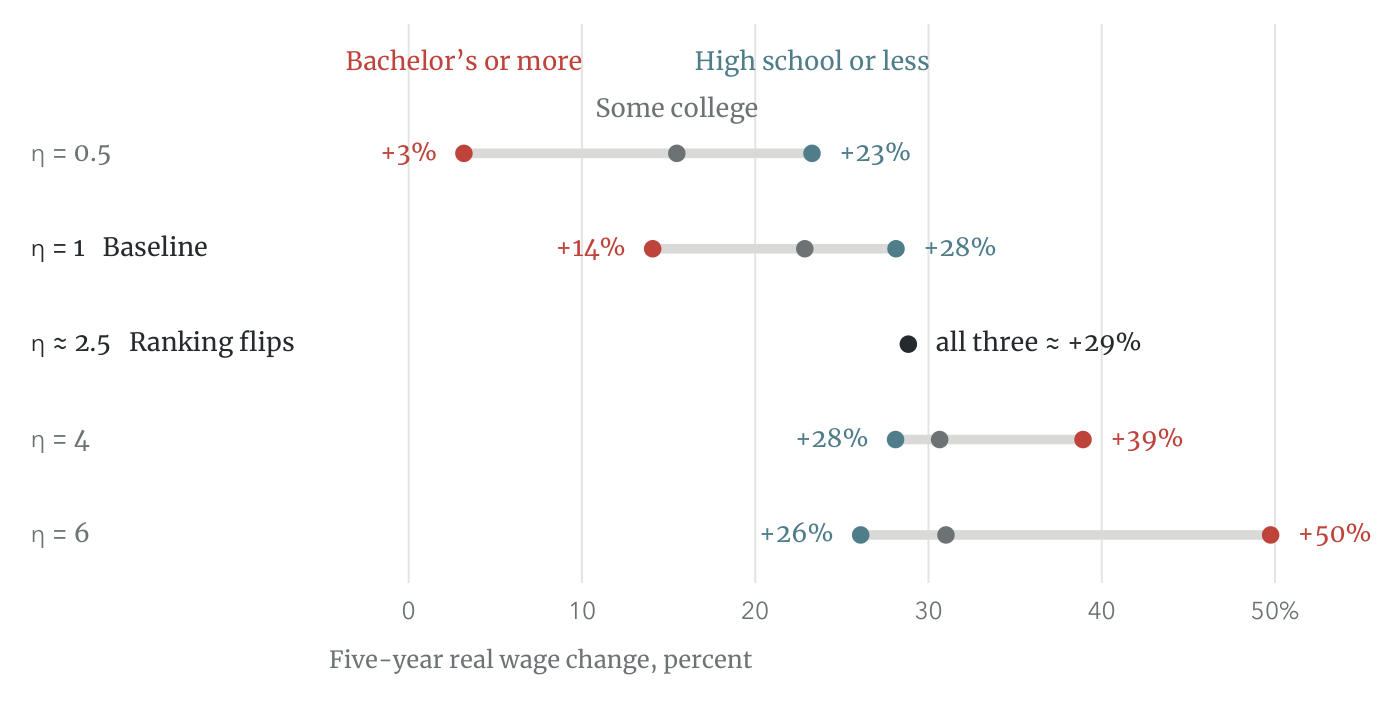
\includegraphics[width=0.98\textwidth]{jevons_tmp/prototype_jevons_figure_all_uses_paper.png}
\vspace{0.25em}
 %
\begin{minipage}[c]{0.94\textwidth}%
{\footnotesize\textit{Notes:}}{\footnotesize{} Five-year real wage gains
by education group under jagged AI adoption, on the central cost path,
with the stock of AI capacity held fixed and workers who move across
sectors at the calibrated $\kappa=1.5$, calculated in the calibrated
model of Section~\ref{sec:counterfactuals} with input--output linkages
and fixed sector-specific capital; the same $\eta$ governs every
use of a sector's output, final and intermediate. The figure reports
the gains for five values of the elasticity of substitution across
sector outputs $\eta$ of Appendix~\href{https://ahmadlp.github.io/Lashkaripour_AI_Displacement_Online_Appendix.pdf\#page=60}{B.10}, equation~\href{https://ahmadlp.github.io/Lashkaripour_AI_Displacement_Online_Appendix.pdf\#page=61}{(B206)},
with $\eta=1$ the paper's Cobb--Douglas baseline. At $\eta\approx2.5$,
workers with a bachelor's degree or more and workers with high school
or less gain the same $28.9$ percent. If the
same elasticity holds only for final demand, the two groups gain the
same at $\eta\approx3.9$. Our calculation
uses the Epoch AI--Ipsos survey, O{*}NET, the BEA industry accounts,
BLS employment, the 2024 American Community Survey, and occupation
exposure ratings~\citep{epochpolling2026,onet2026,bea2026io,bls2026oews,census2024pums,emmr2024}.}%
\end{minipage}
\end{figure}


\section{Conclusion}\label{sec:conclusion}

This paper offers a pro-labor view of explosive AI-driven growth.
The view draws on Ricardo's theory of comparative advantage. An interesting
implication of the theory is that AI displacement coincides with real
wage gains at the aggregate level as long as humans and agentic AI
have different productivity profiles across tasks. More important,
if the difference is sufficiently large and AI adoption is not too
jagged and concentrated in select industries, then every worker can
gain from AI-driven growth, even if they cannot switch sectors. One
reason is a unique feature of AI-driven displacement that distinguishes
it from trade-driven displacement and past episodes of automation:
it leaves some niche tasks to workers within each sector. Engines
displaced horses because they were uniformly more productive than
horses at all tasks, which left horses no niche tasks to retreat to.
Agentic AI may perform every task better than humans, but the relative
difference between humans and agentic AI across tasks is not uniform.

Many commentators have made this argument informally. We formalize
it in a dynamic Ricardian assignment model in which no task is reserved
for humans. As AI becomes more productive, it takes over the tasks
on which it has the greatest cost advantage, and workers retreat into
a narrower set of niche tasks. The real wage then rises in inverse
proportion to labor's share of economic tasks, with an elasticity
that measures the jaggedness of AI capabilities. Because labor's share
of GDP equals its share of tasks, the aggregate real wage effects
of AI are determined by two sufficient statistics, the jaggedness
of AI capabilities and the change in labor's share of GDP, which we
can measure without estimating an aggregate production function. It
follows that the niche tasks left to workers are not expensive bottlenecks;
wages grow instead because workers become more productive on the tasks
they retain and the wage buys a larger basket of goods. The distribution
of comparative advantage governs the pace of wage gains and their
eventual limit, but not the direction. More displacement also amplifies
the marginal wage gains from AI growth, and when fixed shares of output
are allotted to AI installation and research, the real wage rises
without bound on the path to a singularity in finite time.

Across sectors, balanced AI adoption is the worst case scenario for
aggregate real wages, because workers have no lagging sector to retreat
to. When adoption is jagged, labor concentrates in lagging sectors
and commands a wage proportional to their price, which rises relative
to the economy-wide price index through rapid AI-driven growth elsewhere.
If adoption eludes some sectors, real wages grow at the same rate
as output. Input-output linkages raise the share of output growth
appearing as wage growth under balanced adoption. Even when workers
cannot switch sectors, real wages benefit from AI growth across the
board unless AI adoption is extremely jagged across industries. Trade-driven
displacement immiserated workers in import-competing sectors because
trade is concentrated in select industries and operates under a high
trade elasticity.

We estimate $\psi$, the parameter that reflects the jaggedness of
AI capabilities, from the cost of humans versus AI on similar software
engineering tasks. By the end of the sample, AI completes $75.2$
percent of the tasks below human cost. Our two estimation methods
yield $\psi=1.14$ and $\psi=1.36$, so
each percent decline in labor's share of GDP raises the real wage
by $0.7$ to $0.9$ percent. We view
these estimates as a plausible upper bound on the economy-wide $\psi$,
because AI's productivity is likely to be more dispersed across tasks
outside software engineering, so our quantitative results are conservative.
The calibrated model is not rejected by a test against the recent
effects of AI growth on sectoral wages, which were not targeted in
the calibration, whether workers remain in their original sectors
or move across sectors.

If AI continues to grow along the same trajectory, average real wages
rise by $18.5$ percent
after five years, while labor's share of GDP falls from $54.1$
to $39.9$ percent. With an
AI frontier five times less jagged, real output rises by more, but
average real wages rise by only $0.64$
percent. At about the same output growth, jagged adoption pays workers
more than balanced adoption. Every education group gains, even when
workers cannot move across sectors, with five-year gains that range
from $12.5$ percent for workers with a
bachelor's degree or more to $31.2$ percent
for those with high school or less. The Jevons paradox, in which the
knowledge workers that AI displaces gain the most, emerges only if
the elasticity of substitution across sectors exceeds about $2.5$.

Our analysis has several caveats. To isolate the pure impact of AI-driven
growth through Ricardian comparative advantage, we shut down all other
engines of growth, including population growth and capital investment,
even though fertility rates and investment decisions are presumably
influenced by AI-driven growth. Ricardian reassignment is also not
the only force affecting labor market outcomes. Our estimates of jaggedness,
drawn from software engineering tasks, describe observed comparative
advantage and do not determine its ultimate range. Deriving the shares
of output allotted to AI installation and research from equilibrium
investment decisions, and estimating the jaggedness of AI capabilities
outside software engineering, are left for future work. \label{main-text-end}

\begin{singlespace}

\bibliographystyle{aea-insights}
\bibliography{references}

\end{singlespace}
\end{document}
